%%
%
% ARQUIVO: main.tex
%
% VERSÃO: 1.0
% DATA: Maio de 2016
% AUTOR: Coordenação de Trabalhos Especiais SE/8
% 
%  Arquivo tex principal do documento de Projeto de Fim de Curso (PFC).
%  Este arquivo SÓ PRECISA SER MODIFICADO NA PARTE DE CONTEÚDO:
%
%    a. colocar um \include{•} para cada capítulo do documento de PFC.
%
%%

% -----
% CLASSE DO DOCUMENTO DE PFC
% -----
\documentclass{pfc}

% -----
% PACOTES LATEX USADOS NO DOCUMENTO DE PFC
% -----
\usepackage[brazilian]{babel}
\usepackage[utf8]{inputenc}
\usepackage[T1]{fontenc}

\usepackage{amsmath}
\usepackage{graphicx}
\usepackage{tabularx}
\usepackage{float}
\usepackage{color}
\usepackage{amsfonts,amssymb}
\usepackage[authoryear]{natbib}

\usepackage{enumitem}
\usepackage{rotating}
\usepackage{lipsum}
\usepackage{lastpage}
\usepackage{stringstrings}
\usepackage{pgffor}

\usepackage{pgfgantt} %for tikzpicture
\usepackage{xfrac} % for maths
\usepackage{lscape} % enable landscape page
 \usepackage{multirow} %enable cell spanning in multiple rows
% -----
% MARGENS DO DOCUMENTO DE PFC
% -----
\usepackage{geometry}
\geometry{
	a4paper,
	total={210mm,297mm},
	left=25mm,
	right=25mm,
	top=25mm,
	bottom=30mm,
	textwidth=160mm,
	textheight=242mm,
	headheight=0mm,
	headsep=0mm,
}

% -----
% DECLARAÇÕES AUXILIARES PARA REFERÊNCIAS
%
%  Diferencia \citet e \citep de acordo com a NBR 10520:2002
% -----
\DeclareRobustCommand{\NATand}{;}
\DeclareRobustCommand{\NATetal}{et~al.}
\makeatletter
\renewcommand{\NAT@nmfmt}[1]{%
  \ifNAT@swa\expandafter\MakeUppercase
  \else\DeclareRobustCommand{\NATand}{ e}\expandafter\@firstofone\fi{{\NAT@up #1}}%
}
\makeatother

% -----
% AMBIENTE DE FIGURAS DE PFC
%
%  A classe do documento está configurada SOMENTE para figuras no formato EPS.
%  Logo, use PREFERENCIALMENTE este tipo de arquivo.
%
%    a. os arquivos das figuras devem estar no diretório 'img'
% -----
\graphicspath{{./img/}}

% -----
% INÍCIO DO DOCUMENTO DE PFC
% -----
\begin{document}

% -----
% PARTE PRÉ-TEXTUAL DE PFC
%
% Alterar o CONTEÚDO dos arquivos siglas.tex E pre-texto.tex
% -----
%%
%
% ARQUIVO: dados-pfc.tex
%
% VERSÃO: 1.0
% DATA: Maio de 2016
% AUTOR: Coordenação de Trabalhos Especiais SE/8
% 
%  Arquivo tex com os dados acerca do documento de PFC e da apresentação.
%
%   nos campos que definem nomes (autor; orientador; co-orientador; membros da banca)
%   É PRECISO usar os COMANDOS LaTeX para acentuação, conforme abaixo:
%
%         \'a - á || \`a - à || \~a - ã || \^a - â 
%         \'e - é || \^e - ê || \'i - í 
%         \'o - ó || \~o - õ || \^o - ô 
%         \'u - ú || \"u - ü
%
%%

%%% AUTORES DO PFC (Nome completo)
% ---
%  aceita até 03 autores (de autorI até autorIII)
%    a. preencher sucessivamente a partir de autorI
%    b. REMOVER as definições não necessárias
% ---
\autorI{Jonas Rocha Lima Amaro}
\autorII{Yago Guimar\~aes Coimbra}
%\autorIII{Nome Completo do Terceiro Autor}

%%% POSTOS DOS AUTORES DO PFC
% ---
%  aceita os postos de até 03 autores (de postoautorI até postoautorIII)
%    a. preencher sucessivamente a partir de postoautorI (que deve ser o posto de autorI)
%    b. se o autorX É CIVIL, NÃO DEFINIR postoautorX (remover a linha de definição)
%    c. se o autorX É MILITAR, DEFINIR postoautorX com UMA das seguintes ALTERNATIVAS: Alu / 1 Ten / Cap
% ---
%\postoautorI{1 Ten}
%\postoautorII{Alu}
%\postoautorIII{Cap}

%%% TITULO DO PFC
\titulo{Ferramenta para Detecção de Padrões de Botnet Baseado em Algoritmos de Agrupamento de Aprendizagem de Máquina}

%%% DATA DA APRESENTAÇÃO (formato {dd}{Mmmmm}{aaaa})
\datadefesa{01}{Agosto}{2016}

%%% ORIENTADOR DO PFC
% ---
%  CAMPO 1: P (para Prof.); PA (para Profa.); ou qualquer coisa (inclusive VAZIO) - o que for escrito aparecerá no documento
%  CAMPO 2: Nome completo
%  CAMPO 3: D (para D.Sc.); P (para Ph.D.); M (para M.Sc.) ou qualquer coisa (inclusive VAZIO) - o que for escrito aparecerá no documento
%  CAMPO 4: Instituição (com "do / da")
% ---
\orientador{P}{Sergio dos Santos Cardoso Silva}{D}{do IME}

%%% CO-ORIENTADOR DO PFC
% ---
%  se não houver co-orientador, REMOVA ESTA LINHA
%  preenchimento idêntico a \orientador{}{}{}{}
% ---
%\coorientador{P}{Nome Completo do Co-orientador}{P}{do IME}

%%% NÚMERO DA ENTRADA DA BIBLIOTECA (pegar na Biblioteca do IME)
\biblioref{004.69}{S586e}

%%% PALAVRAS-CHAVES DO PFC
% ---
%  devem ser separadas por vírgula e É OBRIGATÓRIO ter pelo menos uma
% ---
\palavraschaves{Botnets, Bots, Detecção de Botnets, Aprendizagem de Máquinas, Clustering, Detecção de Anomalia}

%%% OUTROS MEMBROS DA BANCA DO PFC
% ---
%  aceita até mais 05 membros (de membrobancaI até membrobancaV)
%    a. preencher sucessivamente a partir de membrobancaI
%    b. REMOVER as definições não necessárias
%
%  cada membro tem preenchimento idêntico a \orientador{}{}{}{}
% ---
\membrobancaI{PA}{Raquel Coelho Gomes Pinto}{D}{do IME}
\membrobancaII{P}{Julio Cesar Duarte}{D}{do IME}
%\membrobancaIII{}{Nome do Membro da Banca 3}{}{da COPPE/UFRJ}
%\membrobancaIV{}{Nome do Membro da Banca 4}{}{da UNIRIO}
%\membrobancaV{}{Nome do Membro da Banca 5}{}{da UERJ}

%%
%
% ARQUIVO: pre-texto.tex
%
% VERSÃO: 1.0
% DATA: Maio de 2016
% AUTOR: Coordenação de Trabalhos Especiais SE/8
% 
%  Arquivo tex para a criação da parte pré-textual do documento de Projeto de Fim de Curso.
%
%%


% -----
% PÁGINA DE CAPA DO DOCUMENTO DE PFC
% -----
\makecapa

% -----
% PÁGINA DE TÍTULO DO PFC
% -----
\prepareadvisors
\maketitle

% -----
% PÁGINA DE CRÉDITOS DO DOCUMENTO DE PFC
% -----
\makecredits

% -----
% PÁGINA DE FOLHA DE ASSINATURAS
% -----
\preparemembers
\approvalpage

% -----
% PÁGINA DE DEDICATÓRIA (OPCIONAL, ie. pode remover toda a página)
% -----
%%% DEDICATÓRIA - PREENCHER...
%\dedicatoria{%
%Ao Instituto Militar de Engenharia, alicerce da minha formação e aperfeiçoamento.
%}%
%\makededication

% -----
% PÁGINA DE AGRADECIMENTOS (OPCIONAL, ie. pode remover toda a página)
% -----
%%% AGRADECIMENTOS - PREENCHER...
\agradecimentos{%
Ao Professor Orientador Sergio dos Santos Cardoso Silva por sempre exigir o nosso melhor, pelo seu apoio e conhecimento compartilhado.\\
\indent
Aos nossos amigos e colegas que sempre estiveram do nosso lado, nos auxiliando a superar as dificuldades e compartilhando nossos momentos de felicidade.\\
\indent
As nossas famílias que sempre nos deram força e entenderam as ausências necessárias para que percorrêssemos essa longa, porém gratificante jornada.  \\
}%
\makethanks

% -----
% PÁGINA DE EPÍGRAFE (OPCIONAL, ie. pode remover toda a página)
% -----
%%% EPÍGRAFE - PREENCHER...
\epigrafe{%
Se é previsto que uma máquina seja infalível, ela não pode ser também inteligente.
}%
\autorepigrafe{%    %% Se não tem autor, coloque "Anônimo"
Alan Turing
}%
\makeepigraph

% -----
% PÁGINA DE SUMÁRIO
% -----
\tableofcontents

% -----
% PÁGINAS DE LISTAS DE FIGURAS E DE TABELAS
% se o documento de PFC não possui figuras e/ou tabelas, REMOVA O COMANDO CORRESPONDENTE
% -----
\listoffigures
\listoftables

% -----
% PÁGINA DE LISTA DE SIGLAS
% se o documento de PFC não possui siglas, REMOVA TODA A PÁGINA
% -----
%%% SIGLAS - PREENCHER...
\acronimo{EB}{Exército Brasileiro}
\acronimo{C\&C}{Comando e Controle}
\acronimo{IRC}{Internet Relay Chat}
\acronimo{HTTP}{HyperText Transfer Protocol}
\acronimo{P2P}{Peer-to-peer}
\acronimo{IDS}{Intrusion Detection System}
\acronimo{DNS}{Domain Name System}
\acronimo{CDCiber}{Centro de Cibernética}
\acronimo{IDE}{Integrated Development Environment}
\acronimo{FBE}{Fluxo Básico de Eventos}

\listofnicks

% -----
% PÁGINA DE LISTA DE ABREVIATURAS
% se o documento de PFC não possui abreviaturas ou símbolos, REMOVA TODA A PÁGINA
% -----
%%% ABREVIATURAS - PREENCHER...
%\abreviatura{Ja}{jacobiano}
%\abreviatura{JS}{fluxo secundário (difusivo)}
%\abreviatura{M}{número de Mach}

%%% SÍMBOLOS - PREENCHER...
%\simbolo{$\Phi$}{termo de dissipação viscosa}
%\simbolo{$\Gamma$}{coeficiente de difusão efetivo}
%\simbolo{$\alpha$}{fator de sub-relaxação}
%\simbolo{$\phi$}{variável dependente da equação diferencial geral}

%\listofsymbols

% -----
% PÁGINA DE RESUMO
% -----
%%% RESUMO - PREENCHER...
\resumo{%
Botnets são uma ameaça cibernética que já causou muito prejuízo \citep{silva2013botnets}. Essa ameaça utiliza computadores infectados para realizar atividades fraudulentas como servir páginas piratas para roubar informações sensíveis, enviar \textit{spam} para usuários comuns e enviar sucessivas requisições para derrubar servidores. Por ser uma atividade ilegal, os criminosos realizam a comunicação entre as máquinas com comportamentos divergentes. Essa é uma questão de grande importância para o Exército Brasileiro, uma vez que em 2008 foi aprovado um decreto que determina a Defesa Cibernética um dos setores prioritários para o exército brasileiro\\
\indent
Baseado nessa premissa, esse projeto se propõe a auxiliar na detecção de máquinas que pertencem à botnets utilizando algoritmos de Aprendizado de Máquina da classe de Agrupamento. Dentro dos grupos identificados, espera-se que apareçam grupos pequenos, nos quais estarão as máquinas suspeitas de pertencerem à botnets e que devem ser investigadas. \\
\indent
Dentro do contexto Exército Brasileiro, o projeto auxiliará a Inteligência do Exército Brasileiro na prevenção de ataques por botnets. Dado que, esse sistema aspira fazer parte do raciocinador para um sistema que desarticula botnets. Mais especificamente, será uma ferramenta que filtrará o fluxo da rede para possibilitar que o usuário consiga dar atenção às máquinas de fato suspeitas. Além disso, o sistema deverá auxiliar o analista a entender o que caracterizou tais máquinas como suspeitas.
}%
\makeresumo

% -----
% PÁGINA DE ABSTRACT
% -----
%%% ABSTRACT - PREENCHER...
\abstract{%
Botnets are a cyber threat that already brought plenty of money dispend \citep{silva2013botnets}. This threat uses infected computers to perform fraudulent activities, such as serving pirated sites to steal sensible information, sending spam to common users and sending successive requests to get servers down. Because it is an illegal activity, the criminals do the communication between the machines with divergent behaviours. This matter is a great issue for the brazilian army, because in 2008 a decret was approved that makes Cyber Defence one of the army's top priorities.\\
\indent
Based on that premise, this project proposes to detect machines that are part of a botnet using Clustering, a type of Machine Learning algorithm. Within the identified clusters, it is expected that some will be small, in which the machines suspected to belong to botnets and that deserve to be investigated are expected to be.\\
\indent
Inside the Brazilian Army context, the project will help the Brazilian Army Intelligence preventing botnet attacks. This system aspires to be an important piece of an integrated botnet desarticulating system. More specifically, it will be a tool that filters the network stream in order to make possible to an user pay attention to the actual suspect machines. Besides that, the system must help the user to understand what made those machines suspect.
}%
\makeabstract


\parindent 0.75cm

% -----
% PARTE DE CONTEÚDO DE PFC
%
%  Escrever cada capitulo do documento de PFC em um arquivo .tex separado.
%  Adicionar os arquivos .tex ao documento com comando \include{•}
% -----

\chapter{Introdução}
O espaço cibernético sofre com um crescente número de ataques maliciosos. Esse fato faz com que a pesquisa na área de defesa cibernética ganhe muita importância. Ademais, novas formas de ataques cibernéticos são criadas e antigas são atualizadas, dificultando o objetivo de livrar nossas máquinas de qualquer ameaça \citep{bharathula2016equitable}. Uma dessas formas de ameaças, responsável por grande parte dos ataques em larga escala pela Internet atualmente, é formada pelas botnets.

As botnets, que são redes formadas por máquinas infectadas por alguma forma de \textit{malware}, apresentaram um elevado crescimento no início do século XXI, se tornando uma das ameaças mais desafiadoras no campo de defesa cibernética \citep{chang2015measuring}. A detecção dessas redes se tornou um tópico muito importante na área de defesa cibernética, devido ao desafio que é realizar essa detecção, pois, as botnets são muito flexíveis e robustas, além de estarem em processo de aprimoramento contínuo \citep{bu2010new}.

Com a necessidade de realizar essa detecção, mesmo com as mudanças realizadas no funcionamento das botnets ao longo do tempo, o emprego de técnicas de aprendizado de máquina é muito promissor, especialmente as técnicas de agrupamento. É esperado que os bots que formam as botnets, tenham comportamento diferente de usuários convencionais, e, dessa forma, espera-se que eles sejam agrupados em grupos menores dos formados pela massa de usuários normais.

Levando em conta essas características, o presente trabalho busca desenvolver uma ferramenta para auxiliar na detecção de botnets, utilizando as informações das consultas ao servidor DNS realizadas na rede através de algoritmos de aprendizado de máquina.

\section{Objetivo}
O objetivo deste trabalho é desenvolver uma ferramenta para auxiliar na detecção de possíveis hospedeiros de bots em uma botnet, reduzindo o trabalho humano utilizado na detecção das botnets. Isso será feito utilizando algoritmos de agrupamento, que utilizarão dados que serão calculados através das informações contidas em consultas de DNS realizadas. 

Além disso, o desempenho dessa ferramenta será avaliado, utilizando as informações do log de DNS dos servidores do IME, para o qual já temos algumas máquinas infectadas previamente mapeadas por inspeção e investigação manuais.

\section{Motivação}
O crescimento e diversificação do uso da Internet, criaram o cenário ideal para o desenvolvimento das botnets, que são consideradas uma das maiores ameaças atuais na área de segurança da informação \citep{ji2008botnet}. 

Esta ameaça requer uma atenção especial, principalmente no âmbito militar, devido à aplicação que as botnets podem ter no contexto de defesa cibernética, permitindo que os atacantes inutilizem servidores do inimigo e/ou coletem informações confidenciais.

A detecção das botnets é um grande desafio, pois os atacantes estão sempre aprimorando o funcionamento dos bots, e com isso, os mecanismos atuais muitas vezes falham ao detectar novas implementações de botnets. Isso motivou o uso de algoritmos de agrupamento para serem utilizados na detecção de botnets, de forma que a ferramenta seja capaz de detectar inclusive botnets que sejam desconhecidas.

Por esses motivos, torna-se muito clara a necessidade da criação de uma ferramenta que permita facilitar o trabalho de detecção de novas botnets, não previstas pelas ferramentas atuais, já que novas botnets só poderiam ser identificadas por inspeção manual, que é um processo bastante complexo devido à enorme quantidade de informações presentes em uma rede.

\section{Justificativa}
A justificativa desse trabalho é contribuir para a área de defesa cibernética, uma área de interesse do IME e do Exército Brasileiro (EB), uma vez que em 2008 foi aprovado um decreto que determina essa área como um dos setores prioritários para o EB. apoiando à pesquisa com o conhecimento de características de consultas de DNS que podem ser relevantes para realizar a detecção de botnets. Além disso, a ferramenta pode ser utilizada pelo Centro de Defesa Cibernética (CDCiber) ou servir como um módulo de um sistema integrado de detecção de botnets \citep{silva2012arquitetura}, auxiliando na investigação de atividades suspeitas nas redes.

\section{Metodologia}
Este trabalho foi dividido em cinco fases principais: estudo teórico, preparação dos dados, implementação dos algoritmos de agrupamento aos dados preparados, breve análise e testes dos resultados e implementação da interface gráfica. 

Na etapa de estudo teórico foi feito um levantamento da funcionalidade das botnets e do funcionamento e aplicações dos algoritmos de aprendizado de máquina, com o objetivo de identificar vulnerabilidades e padrões nas botnets, motivando a seleção de características relevantes dos dados utilizados, de forma a melhorar a performance do algoritmo.

Na etapa seguinte, foi feito um levantamento das características candidatas a serem utilizadas pelo algoritmo da ferramenta. De posse dessas características, foi implementado um programa em C++ para realizar a extração automática dessas características da base de dados que utilizamos.

Na etapa de implementação dos algoritmos de agrupamento aos dados preparados, utilizamos a ferramenta \textit{Scikit-Learn} para desenvolvermos um programa escrito em Python que aplica algoritmos de aprendizado de máquina nas características previamente levantadas.

Posteriormente, foi feita uma breve análise, para identificar as técnicas mais adequadas, possíveis refinamentos na ferramenta e comprovar sua eficiência na detecção de bots.

Por fim, foi implementada uma interface gráfica para facilitar o uso da ferramenta pelos usuários, integrando todos as funcionalidades desenvolvidas em uma aplicação multi-plataforma utilizando a ferramenta \textit{Qt Creator}.

\section{Estrutura}
Este trabalho é composto por sete capítulos, iniciando com esta introdução. No capítulo 2 é feito um estudo teórico sobre botnets para identificar o tipo de \textit{malware} que desejamos identificar. Em seguida, no capítulo 3, é realizado um estudo sobre algoritmos de aprendizado de máquina dando ênfase nos algoritmos de agrupamento, que será a estratégia utilizada neste trabalho. Em seguida, no capítulo 4, são explicados os procedimentos e a motivação que levaram à forma de tratamento dos dados. O capítulo 5 mostra quais foram os resultados preliminares encontrados, fazendo uma análise sobre as características dos grupos formados, mostrando as motivações para os próximos aprimoramentos. No capítulo 6, são mostradas as funcionalidades do sistema desenvolvido com a interface gráfica e como foi feita sua arquitetura. Ao final, no capítulo 7, estão as conclusões que foram obtidas ao longo do desenvolvimento da ferramenta.
\chapter{Botnets}
As Botnets são redes formadas por máquinas infectadas com malware, permitindo que o atacante (\textit{botmaster}) realize diversas atividades criminais remotamente, como roubo de informações, ataques de negação de serviço, envio de SPAM, etc.\cite{silva2013botnets}

Com o crescimento e diversificação do uso da Internet, o meio cibernético se tornou mais relevante e mais atraente para a realização de ataques maliciosos. Isso motivou o crescimento do número de botnets existentes e aumentou o potencial de contaminação das mesmas, além disso, para evitar os mecanismos de detecção existentes, elas se tornaram cada vez mais sofisticadas.

Para que o detector se torne mais robusto, é preciso compreender o funcionamento das botnets e seus objetivos. Esse conhecimento é necessário para entender as configurações existentes nas botnets atuais, além de compreender como essas configurações podem evoluir. De posse desse conhecimento, espera-se que seja possível identificar características relevantes e intrínsecas ao funcionamento das botnets, mesmo quando o \textit{botmaster} estiver tentando evitar os mecanismos de detecção.

\section{Elementos das Botnets}
As botnets apresentam alguns elementos estruturais tipicamente envolvidos, que estão presentes independente do protocolo ou arquitetura utilizada. A Figura \ref{fig:typical_elements} mostra a estrutura desses elementos e como eles se relacionam em uma botnet. Segue uma descrição para cada componente:
\begin{itemize}  
\item Bots: São malwares instalados nos computadores das vítimas que podem realizar as ações maliciosas que o \textit{botmaster} envia através do canal de comando e controle (C\&C). Geralmente, o malware é inicializado quando o hospedeiro inicializa a máquina, porém isso pode ser configurado pelo \textit{botmaster} para dificultar a detecção da atividade maliciosa.
\item Hospedeiros (Zumbis): São as máquinas em que o bot foi instalado, ou seja, infectadas.\cite{puri2003bots}
\item \textit{Botmaster}: é o indivíduo que configura o bot, dissemina e controla a botnet.
\item Canal de Comando e Controle (C\&C): é o meio que o \textit{botmaster} tem para se comunicar com a sua botnet. É a parte chave do funcionamento, pois é necessário para o envio dos comandos de atividade maliciosa aos hospedeiros. Dessa forma, grande parte das características da botnet, como robustez, facilidade de detecção/desativação, estabilidade, etc., são definidas pela forma que a infraestrutura de C\&C está organizada.
\end{itemize}

\begin{figure}
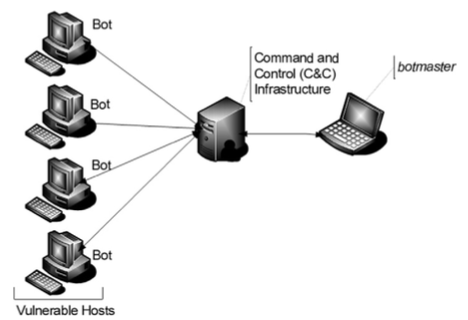
\includegraphics[width=\textwidth]{typical_elements}
\caption[Elementos das botnets]{Elementos das botnets \cite{silva2013botnets}} \label{fig:typical_elements}
\end{figure}

\section{Ameaças e Formas de Defesa}
O crescimento do número de máquinas conectadas constantemente a enlaces de alta velocidade e rodando sistemas com vulnerabilidades consideráveis, criou um ambiente favorável à formação de botnets. Além disso, muitas vezes o bot é transparente ao responsável pela máquina infectada, ou seja, não atrapalha o funcionamento da máquina, fazendo com que a vítima não perceba a infecção e tente combatê-la. Esses fatores, aliados ao enorme potencial de causar danos, fazem com que as botnets sejam um dos maiores desafios de pesquisa em segurança no espaço cibernético atual. \cite{soltani2014survey}

Existem características que tornam o host mais interessante ao \textit{botmaster} como: altas taxas de transmissão, baixos níveis de segurança e monitoração, alta disponibilidade e localização distante (dificultando que as agências reguladoras detectem as atividades, já que os bots estarão espalhados por diversas nações). Esses fatores ajudam o bot a passar desapercebido e a contribuir com maior capacidade de banda ao \textit{botmaster}, facilitando ataques como os de negação de serviço.

Existem duas formas para combater um ataque realizado por botnets: reativamente ou preventivamente. A forma reativa é a mais comum e envolve detectar a existência da atividade maliciosa e reagir ao ataque tentando reduzir o tráfego malicioso para níveis aceitáveis. Uma desvantagem é que o ataque já vai ter sido inicializado quando for detectado, ou seja, já vai haver causado danos antes de ser solucionado. A forma preventiva busca evitar que a botnet possa realizar alguma atividade maliciosa, porém essa atividade não é simples, já que o atacante pode aprimorar seus bots, tornando-os mais sofisticados, exigindo grandes investimentos para manter os recursos de segurança atualizados.

O mecanismo que estamos desenvolvendo é da forma preventiva, já que o algoritmo busca encontrar padrões e identificar possíveis máquinas infectadas por botnets. Tudo isso na fase de disseminação da botnet, ou seja, antes do atacante realizar um ataque, como negação de serviço, por exemplo. Uma característica desejável para um detector é a detecção em tempo real, com o objetivo de minimizar os danos causados e o tempo de reação do \textit{botmaster}. Porém, obter essa característica é um desafio, devido ao grande número de dados que devem ser tratados e analisados. Dessa forma, nosso projeto não fará detecção em tempo real, mas tentará se aproximar disso, utilizando a detecção dos dados coletados ao longo de um dia para detectar bots que atuaram nas últimas 24 horas.

\section{Ciclo de Vida das Botnets}
Na maioria dos casos, existe um ciclo com fases bem definidas de como uma botnet é criada e mantida, a Figura \ref{fig:botnets_lifecycle} mostra essas fases para cada novo hospedeiro que é contaminado.

\begin{figure}
\tikzstyle{block} = [rectangle, draw, text width=9em, text centered, rounded corners, minimum height=4em]
\tikzstyle{line} = [draw, -latex']
\centering
\begin{tikzpicture}[node distance = 4.5cm, auto]
    % Place nodes
    \node [block] (init) {Infecção Inicial};
    \node [block, below of=init] (second) {Injeção Secundária};
    \node [block, right of=init] (connection) {Conexão};
    \node [block, below of=connection] (malicious) {Atividades Maliciosas};
    \node [block, right of=malicious] (update) {Manutenção e Atualização};
    % Draw edges
    \path [line] (init) -- (second);
    \path [line] (second) -- (connection);
    \path [line] (connection) |- +(4,2) |- (connection.east); 
    \path [line] (connection) -- (malicious);
    \path [line] (malicious) -- (update);
    \path [line] (update) -- (connection);

\end{tikzpicture}
\caption[Ciclo de Vida das Botnets]{Ciclo de Vida das Botnets} \label{fig:botnets_lifecycle}
\end{figure}

Na primeira fase, chamada de injeção inicial, o atacante procura vulnerabilidades na máquina do futuro hospedeiro para explorá-las e infecta-lo com o malware, tornando-se um bot em potencial, isso pode ocorrer, por exemplo, através de um download indesejado ou através de um anexo em um e-mail. Após a infecção ser bem sucedida, ocorre a injeção secundária: o host infectado, através do malware inicial instalado, busca em uma rede os reais binários do malware do bot, os quais após baixados e executados concluirão a infecção e tornam o host em um bot real.\cite{feily2009survey}.

Durante a fase de conexão, o bot estabelece conexão com o canal de C\&C, isso se repete sempre que o host é reiniciado, podendo ser considerada uma fase vulnerável já que segue um padrão. Após a efetivação da conexão, o bot se torna ativo na botnet, e passa a realizar os comandos enviados pelo \textit{botmaster} através do canal de C\&C, efetivando as atividades maliciosas solicitadas. A última fase é a de manutenção e atualização, e tem por objetivo manter a botnet ativa e atualizada, já que se o \textit{botmaster} deseja que os bots possam evitar novas técnicas de detecção, adicionar novas funcionalidades ou até mesmo alterar o servidor de C\&C, os binários do programa bot devem ser modificados.

\section{Arquitetura das Botnets}
Existem 4 tipos de arquiteturas para as botnets: centralizada, descentralizada, híbrida e aleatória. 

Na arquitetura centralizada, mostrada na Figura \ref{fig:centralized_architecture} todos os bots se comunicam com um número pequeno de servidores de C\&C, embora ela ofereça vantagens ao \textit{botmaster}, como baixa latência e facilidade de manutenção, ela também torna a botnet bastante vulnerável, permitindo que ela seja desligada após a identificação dos poucos pontos centrais de C\&C. Ela é muito utilizada pelo protocolo IRC (\textit{Internet Relay Chat}), porém pelo fato de tráfego desse protocolo ser incomum e raramente utilizado, ele costuma ser bloqueado, inutilizando a botnet. Por isso, o uso do protocolo HTTP (\textit{HyperText Transfer Protocol}) se popularizou já que ele é muito utilizado, disfarçando as comunicações das botnets.

\begin{figure}
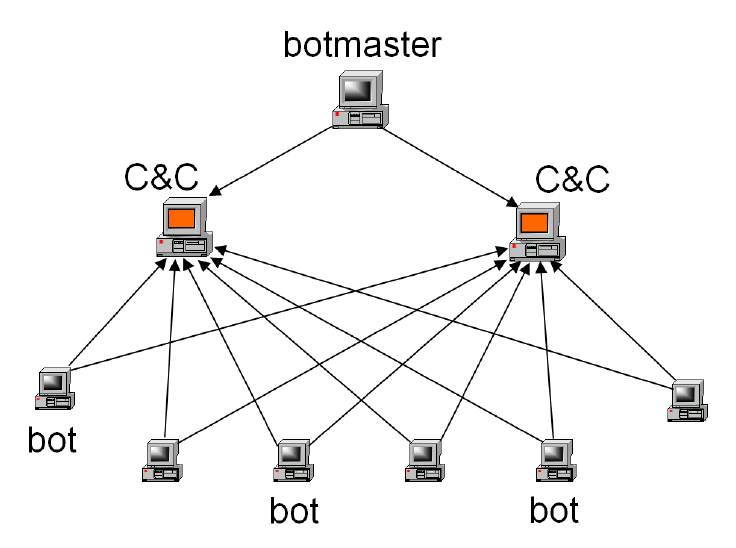
\includegraphics[width=\textwidth]{centralized}
\caption[Arquitetura Centralizada]{Arquitetura Centralizada\cite{wang2010advanced}} \label{fig:centralized_architecture}
\end{figure}

A fragilidade da arquitetura centralizada, motivou o desenvolvimento da arquitetura descentralizada, na qual uma variedade de protocolos P2P (\textit{Peer-to-peer}) é utilizada. A flexibilidade e robustez dessa arquitetura, permite que mesmo que muitos bots sejam desativados a botnet possa continuar funcionando, já que não existem pontos centralizados de C\&C. 

As arquitetura híbridas apresentam características de ambas as arquiteturas centralizadas e descentralizadas, como mostrado na Figura \ref{fig:hybrid_architecture}, na qual os bots são classificados em dois grupos: clientes e servos. Os servos exercem os papéis tanto de clientes quanto servidores, possuindo endereço de IP estático e público para serem acessíveis globalmente, sendo utilizados para repassar os comandos enviados pelo \textit{botmaster}. Os demais bots, são denominados clientes pois não aceitam comunicações de entrada, dessa forma e podem apresentar IP dinâmico, privado ou protegidos por \textit{firewall} para não serem roteados facilmente. Por fim, a arquitetura aleatória é um modelo até agora teórico, no qual o bot não se comunica ativamente com o \textit{botmaster} ou com outros bot, para realizar um ataque o \textit{botmaster} vasculha a rede em busca de um bot para enviar o comando e realizar as atividades maliciosas.

\begin{figure}
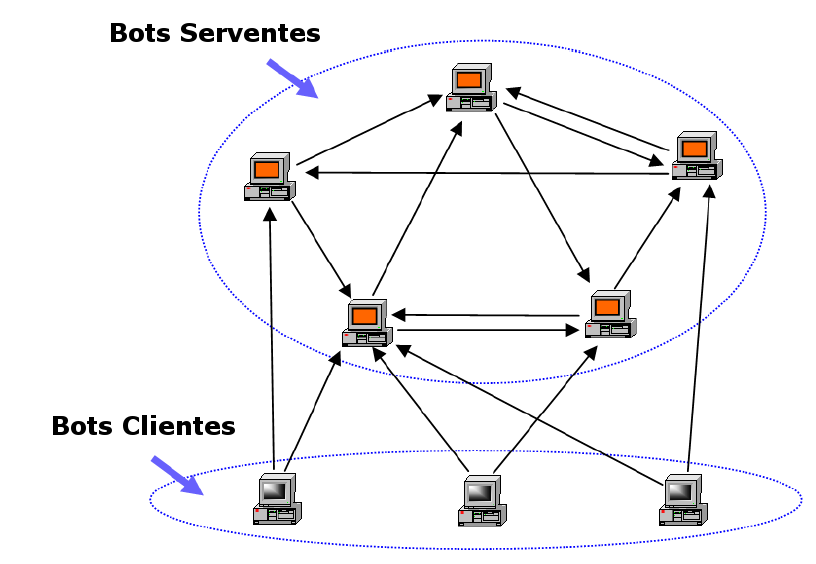
\includegraphics[width=\textwidth]{hybrid}
\caption[Arquitetura Híbrida]{Arquitetura Híbrida\cite{wang2010advanced}} \label{fig:hybrid_architecture}
\end{figure}

\section{Detecção de Botnets}

Existem duas categorias de técnicas para detecção de botnets: \textit{honeynets} e sistemas de detecção de intrusos (IDS). As \textit{honeynets} consistem na criação de redes com a intenção de que elas sejam comprometidas, permitindo que as informações sobre a botnet sejam captadas, por isso elas são consideradas mais efetivas para compreender as características de uma botnet do que a detecção propriamente dita.

A detecção por IDS, pode ser classificada entre duas técnicas: a baseada em assinaturas e a baseada em anomalias. A técnica baseada em assinaturas, consiste em extrair padrões da rede e comparar com um banco de dados onde se encontram os padrões que já foram vistos em botnets, ou seja, ela não permite que novas botnets sejam identificadas e envolve a posse de um banco de dados enorme com o maior número de informações existentes sobre as botnets previamente detectadas. Dessa forma, a técnica baseada em anomalias é a principal área de pesquisa para detecção de botnets, baseando-se em anomalias na rede, como alta latência, aumento no tráfego ou uso de portas incomuns para detectar a presença de bots na rede.

As técnicas baseadas em anomalias, podem ser baseadas no host, onde cada máquina possui uma ferramenta de monitoração instalada (o que não é muito escalável), e tem seu comportamento analisado para verificar a existência de atividades suspeitas. Além disso, a análise pode ser baseada na rede, ativa (que possuem a grande desvantagem de aumentar o tráfego da rede ao injetar pacotes com a finalidade de examinar se um cliente é humano ou um bot) ou passivamente, sendo esta última a forma de detecção mais utilizada e pesquisada atualmente.

A monitoração passiva de uma rede consiste em analisar o tráfego da rede buscando por comunicações suspeitas que podem ter sido enviadas pelos bots ou canais de C\&C. Essa monitoração é possível pois os bots de uma mesma botnet costumam apresentar padrões de comunicação, já que eles são pré-programados pelo mesmo \textit{botmaster} para entrar contato com o servidor de C\&C.

Para que a análise do tráfego seja viabilizada, são empregadas diversas técnicas como métodos estatísticos, mineração de tráfego, teoria de grafos, clustering, modelos estocásticos, redes neurais, entre outras.

A detecção de botnets é uma tarefa bastante desafiadora porque os \textit{botmaster}s estão sempre aprimorando os bots, tornando os mais difíceis de serem detectados. Por exemplo, as primeiras detecções buscavam mensagens suspeitas nos conteúdos da mensagem, afim de evitar isso os \textit{botmaster}s passaram a utilizar criptografia tornando essa técnica de detecção obsoleta. Outra dificuldade para algoritmos de clustering é que podem ser evitados usando técnicas de randomização nas comunicações e atribuição de tarefas diferentes para os bots.


\chapter{Aprendizagem de Máquina}
Como Bishop \cite{bishop2006pattern} descreve, aprendizagem de máquina é uma maneira de abordar um problema de computação. Nessa abordagem, a partir de um grande conjunto de dados, chamados como conjunto de treinamento, são inferidos um conjunto de parâmetros que a serem utilizados em um modelo parametrizado.

\section{Definições}

Algumas breves definições serão apresentadas para fim de ambientar o leitor nos temas discutidos neste capítulo.

\subsection{Amostra}
Seja amostra o conjunto de exemplos que representam os dados conhecidos do problema.

\subsection{Características}
Sejam características um conjunto ordenado de valores que descrevem um exemplo, a ser modelada pelo algoritmo de Aprendizagem.

\subsection{Etiquetas}
Seja etiqueta de exemplo, ou simplesmente etiqueta, a saída esperada do modelo para aquela instância.

\subsection{Avaliações de Desempenho}
Define-se acurácia como:
\[\frac{\mathrm{\#Acertos}}{\mathrm{\#Amostra}}\]

Define-se precisão como:
\[\frac{\mathrm{Verdadeiros Positivos}}{\mathrm{\#Positivos}}\]

Define-se \textit{recall} como:
\[\frac{\mathrm{Verdadeiros Positivos}}{\mathrm{\#Acertos}}\]

Define-se \textit{F1 score} como:
\[\frac{2 * \mathrm{precisão} * \mathrm{recall}}{\mathrm{precisão} + \mathrm{recall}}\]

\subsection{Matriz \(\mathbf{X}\)}
Seja \(\mathbf{X}\), amostra de treinamento, uma matriz \(m \times n\), o qual \(m\) é quantidade de instâncias e \(n\) é a quantidade de características. \(\mathbf{X}\) é a representação matemática da amostra.

\subsection{Vetor \(\mathbf{Y}\)}
Seja \(\mathbf{Y}\), conjunto de etiquetas, um vetor de tamanho \(m\), a quantidade de instâncias, \(\mathbf{Y}\) é o conjunto ordenado das respectivas saídas esperadas de cada linha da matriz \(\mathbf{X}\), ou seja as etiquetas.


\section{Categorias de Problemas}

Para ser mais específico, é possível classificar os problemas resolvidos pela aprendizagem de máquina em cinco categorias\cite{mohri2012foundations}.

\begin{description}
\item \textbf{Classificação}: Decidir a classe de exemplo dadas as suas características, por exemplo decidir qual dígito foi escrito a apartir de uma imagem de dígito escrita a mão.
\item \textbf{Regressão}: Determinar um valor real para cada exemplo, por exemplo o risco de um paciente ter contraído câncer a partir de imagens e resultados de exames.
\item \textbf{Graduação}: Ordenar os exemplos a partir de algum critério, por exemplo listar produtos por relevância a partir das palavras chaves da busca do usuário.
\item \textbf{Aglutinação}: Particionar os exemplos em regiões homogêneas, por exemplo identificar comunidades dentro de redes sociais massivas.
\item \textbf{Redução de Dimensionalidade}: Representar a amostra com número reduzido de dimensões, por exemplo comprimindo imagens para processamento de imagens.
\end{description}

Neste projeto foi decidido encarar o problema como aglutinação, apesar de também poder se confundir com classificação, já que o objetivo é auxiliar a detecção de botnets.

\section{Cenários dos Dados}

Categoriza-se\cite{mohri2012foundations} sete cenários para os algoritmos de aprendizagem, esse cenários são fortemente influenciados pelas condições dos dados de treinamento.

\begin{description}
\item \textbf{Aprendizado Supervisionado}: O modelo tem acesso a dados com e resultados de saída já esperados, ou etiquetados, como lê-se na literatura. Os problemas mais comuns desse tipo de cenários são classificação, regressão e graduação.

\item \textbf{Aprendizado Não Supervisionado}: Só se dispõe da amostra de treinamento sem etiquetas. Geralmente é mais utilizado para classificação, aglutinação e redução de dimensionalidade

\item \textbf{Aprendizado Semi-Supervisionado}: Neste cenário, é possível acessar uma amostra sem etiquetas e uma com etiquetas. Esse é o caso de problemas em que dados sem etiquetas são fáceis de serem adiquiridos, ao contrário dos dados etiquetados, pela dificuldade de etiquetar.

\item \textbf{Inferência Transdutiva}: Semelhante ao Aprendizado Semi-Supervisionado, nem todos os exemplos são etiquetados, mas o modelo só deve ser generalizado apenas para os exemplos conhecidos.

\item \textbf{Aprendizado On-line}: Neste cenário, iterasse no modelo a cada exemplo recebido em rodadas. No início da rodada, o modelo recebe um exemplo, inicialmente sem etiqueta, realiza uma predição, recebe a etiqueta e atualiza os parâmetros do modelo.

\item \textbf{Aprendizado por Reforço}: Neste cenário, os modelos são criados baseado num sistema de recompensa. O modelo é recompensado a cada decisão bem feita ao interagir com um ambiente.

\item \textbf{Aprendizado Ativo}: O algoritmo é quem realiza requisições a uma entidade capaz de etiquetar exemplos para melhorar os parâmetros do modelo. O objetivo é conseguir gerar um modelo tão bom quando o modelo supervisionado, porém com menos exemplos.

\end{description}

E ainda há outras possíveis cenários ainda mais complexos e específicos, não catalogados neste trabalho porque a ciência de Aprendizado de Máquina está ainda em constante fase de crescimento.

\section{Exemplo: Regressão Supervisionada}

Dado um conjunto de tamanho de imóveis e seus respectivos valores de compra em uma vizinhança hipotética estimar o valor de um apartamento sabendo apenas seu tamanho.

Seja o vetor ordenado \(\mathbf{X} = [x_{1},x_{2},...,x_{m}]\), \(\#\mathbf{X} = m\), o tamanho em Metros quadrados de apartamentos em um bairro. Seja \(\mathbf{Y} = [y_{1},y_{2},...,y_{m}]\), o preço do i-ésimo apartamento indexado em \(\mathbf{X}\). Se arranjarmos os valores graficamente obtem-se a Figura 1.

\begin{figure}
	\centering
		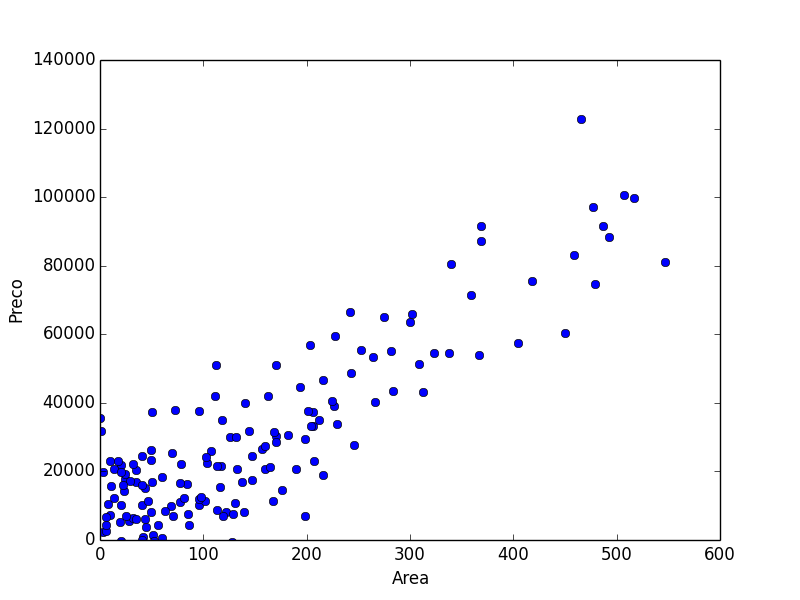
\includegraphics[width=0.9\textwidth]{figure_1.png}
		\caption{a distribuição do preço das casas}
		\label{casas}
\end{figure}

Suponha que de posse do tamanho \(x\), não apresentado em \(\mathbf{X}\), o usuário queira inferir um preço \(y\). Para tal é necessário construir uma hipotese \(h_{\theta}\) que melhor interpole os valores de já conhecidos. Para poder avaliar se \(h_{\theta}\) é ótimo, existe uma função custo, \(custo(h_{\theta},\mathbf{Y})\).

Para esse problema, considera-se:

\[h_{\theta}(x) = \theta_{1}*x + \theta_{0}\]

Ou seja, um modelo linear. Além disso, para avaliar a proximidade do modelo e da amostra, aplica-se o erro quadrádico médio como função custo, isto é:

\[custo(h_{\theta}(X),\mathbf{Y}) = \frac{1}{m}*\sum_{i=1}^{m}(h(x_{i})-y_{i})^2\]

Tem-se dados, função de custo, precisa-se introduzir um método de otimização. Propõe-se, então, o uso Método do Gradiente, que é um método para achar o mínimo local dado um ponto. Como a função de custo em questão é quadrática, ou seja, é convexa. Existe \(\alpha\) tal que atualizando iterativamente os parâmetros \(\theta_{0}\) e \(\theta_{1}\), seguindo a expressão

\[\theta_{0} = \theta_{0} - \alpha * \frac{\partial}{\partial \theta_{0}}  custo(h_{\theta}(X),Y)\]
\[\theta_{1} = \theta_{1} - \alpha * \frac{\partial}{\partial \theta_{1}}  custo(h_{\theta}(X),Y)\]

Converge-se à solução ótima que minimiza o valor da função custo, sendo possível com algum erro inferir o valor do imóvel sabendo seu tamanho. Tal hipótese \(h_{\theta}\) está representado na Figura 2

\begin{figure}
	\centering
		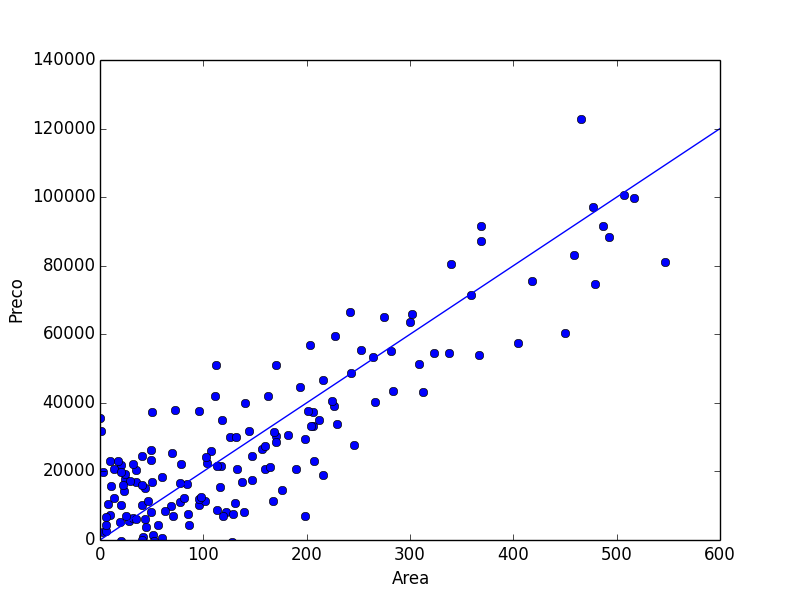
\includegraphics[width=0.9\textwidth]{figure_2.png}
		\caption{o modelo acompanhado e a distribuição do preço das casas}
		\label{casas}
\end{figure}



\section{Detecção de Anomalia}

O artigo, \textit{Anomaly Detection: A Survey}\cite{chandola2009anomaly}, define Detecção de Anomalia o problema da busca por padrões nos dados que não seguem um padrão de um comportamento esperado. Essas anomalias podem acontecer em diversos contextos, ruídos nas medidas, defeitos em equipamentos, comportamentos inovadores ou até atividades fraudulentas, como fraude de cartão de crédito e ataques cibernéticos. Esse tipo de algoritmo pode ser utilizado para resolver problemas de Classificação e Aglutinação.

\subsection{Etiquetas em Detecção de Anomalia}

Geralmente a tarefa etiquetar os dados de modo representativo e preciso é custosa. A forma mais comum de etiquetagem é feita manualmente por um especialista. Esse processo é geralmente custoso, pois são necessários muitos exemplos para encontrar uma anomalia, que por definição é um caso raro. Dentro desse contexto, existem 3 cenários possíveis na operação da Detecção de Anomalias, Supervisionado, Semi-Supervisionado, Não Supervisionado.

Os algoritmos de Detecção de Anomalia Supervisionados convertem têm poucos exemplos de anomalias, por definição, que isso pode trazer problemas quanto a análise da acurácia. O caso extremo seria considerar todos normais e ter acurácia de alta, uma vez que os exemplos anomalos podem representar menos de \(1\%\) da amostra. Isso pode ser resolvido observando a precisão e a exaustividade que resultariam \(0\%\). Como é preciso se chegar em um número para poder comparar performance, Witten\cite{witten2011data} propõe que se avalie o \textit{F1 score}, que seria a média harmônica das duas medidas.

Assume-se que as amostras de treinamento são exemplos etiquetados como normais quando se trabalha no cenário Semi-Supervisionados desse modo é possível criar uma estimativa de como se comportam os exemplos normais e assumir que os que fogem do escopo é anomalia.

Por último, quando não se tem etiqueta para os exemplos opera-se num cenário Não Supervisionado, assume-se que os casos anoma-los são menos frequentes. Note que se essa premissa não for satisfeita, o sistema está sujeito à alta quantidade falsos negativos.

\subsection{Proposta de Modelo}

Será exposto um modelo de Detecção de Anomalia baseado em modelo probabilístico. Suponha que os dados de uma determinada amostra se distribuam no plano determinado pelas características de acordo com o padrão normal. Dessa forma é possível associar cada exemplo \(\mathbf{x}\) à uma probabilidade, \(p(\mathbf{x})\).
Sabe-se\cite{bishop2006pattern} que a distribuição normal multidimensional é

\[\mathcal{N}(\mathbf{x}|\mathbf{\mu},\mathbf{\Sigma})=\frac{1}{(2\pi)^{\sfrac{D}{2}}} \frac{1}{|\mathbf{\Sigma}|^{\sfrac{1}{2}}}\exp\left\{ -\frac{1}{2} (\mathbf{x} - \mathbf{\mu})^T \mathbf{\Sigma}^{-1} (\mathbf{x} - \mathbf{\mu}) \right\}\]

O qual \(D\) é a dimenção de \(\mathbf{x}\), \(\mathbf{\mu}\) é o vetor média de todas as caracteríticas da Matriz \(\mathbf{X}\) e \(\mathbf{\Sigma}\) é uma matriz covariância, \(D \times D\), \(|\mathbf{\Sigma}|\) é seu determinante.

\[\mathbf{\Sigma}=\mathit{cov}[ \mathbf{x} ] = \mathbb{E} \left \lbrack ( \mathbf{x} - \mathbb{E} [ \mathbf{x} ] ) ( x - \mathbb{E} [ \mathbf{x} ] ) ^ T \right \rbrack \]

O qual \(\mathbb{E}\) é o operador valor esperado. Após a construção do modelo probabilístico, o algoritmo decide se tal um novo exemplo \(\mathbf{x}\) é uma anomalia se

\[\mathcal{N}(\mathbf{x}|\mathbf{\mu},\mathbf{\Sigma}) < \varepsilon\]

O qual \(\varepsilon\) é um valor gatilho escolhido previamente que resultou o melhor \textit{F1 score}, se o modelo for aplicado em um cenário Supervisionado.

\chapter{Preparação Dos Dados}
Grande parte dos métodos existentes para detecção de botnets, utilizam informações completas do tráfego da rede, inclusive de informações do \textit{payload} para extrair as características relevantes \citep{krmicek2011inspecting}. Infelizmente, nem sempre todas essas informações estão presentes, por diversos motivos, como: questões de privacidade, falta de autorização para acessar o conteúdo dos pacotes, etc. Por isso, torna-se necessário analisar a capacidade de utilizar informações mais simples, como o fluxo da rede (\textit{NetFlow}) ou o registro do log de requisições a um servidor DNS, para características.

Nesse trabalho vamos focar nos dados das requisições coletadas pelo servidor DNS do IME no período de fevereiro a abril de 2012. Ao longo desse capítulo mostraremos quais as informações contidas nesses registros, as características que consideramos relevantes e como foi feito o tratamento para a extração das mesmas.

\section{Estrutura do Log Bruto de DNS }
O log de DNS utilizado foi baseado nos dados coletados pelo servidor DNS do IME. Esses dados são privados e foram coletados em diversos dias de fevereiro a abril de 2012. Cada registro no DNS é uma requisição que foi feita ao servidor por uma máquina cliente. As informações contidas em cada registro são:

\begin{itemize}
\item Data em que a requisição foi feita
\item Horário com precisão de milésimos da requisição
\item Endereço IP da máquina que fez a requisição
\item Porta do Cliente
\item Nome do domínio requisitado
\item Tipo de Requisição
\item IP do Servidor DNS consultado
\end{itemize}

Abaixo, encontra-se um exemplo de uma entrada no registro de requisições extraído da base de dados: 

\begin{quote}
11-Mar-2012 12:24:16.772 queries: info: client 41.128.225.42\#57135: query: rEcREIo.DE9.iMe.eb.br IN A - (200.20.120.33)
\end{quote}

Dado que os dados não estão estruturados em um formato facilmente reconhecido pelo computador, como em um arquivo JSON ou XML, foi preciso realizar a extração dos dados do log utilizando expressões regulares. A expressão regular foi construída inicialmente para reconhecer alguns exemplos de entradas. Após isso, ela foi aperfeiçoada para reconhecer novos exemplos ao colocar um mecanismo para que o sistema avise quando a entrada não foi reconhecida pela expressão regular. Dessa forma, a expressão era adaptada para reconhecer entradas válidas e que não forem reconhecidas. O mecanismo de aviso foi mantido, afim de garantir o aviso ao usuário de entradas no log que não foram previstas pela expressão regular desenvolvida.

Após aplicar a expressão regular em cada linha extraída do log do servidor DNS do IME, foram filtradas as requisições que foram feitas por máquinas que pertencem à infra-estrutura do IME, como o servidor de correio, já que são seguras e muitas vezes responsáveis por mais de 50\% das entradas no log nos dias analisados. Depois de aplicar esse filtro, o dado tratado pode ser armazenado de modo amigável para a criação do modelo.

\section{A Estrutura do Banco de Dados}
Apenas conseguir fazer a leitura de cada campo do log individualmente não é o suficiente para representar as características que serão utilizadas pelos algoritmos de aprendizado de máquina. Ou seja, elas ainda precisam ser submetidas a diversos cálculos e tratamentos. Com o objetivo de acelerar o processamento desses tratamentos, além de facilitar e agilizar a consulta de informações posteriormente para efetuar uma investigação inicial dos suspeitos levantados pelo sistema, decidimos armazenar as informações em um banco de dados relacional.

O Sistema Gerenciador de Banco de Dados utilizado foi o PostgreSQL, como parte da nossa solução, para facilitar a escrita, leitura e atualização das informações coletadas dos registros DNS. Na modelagem feita, utilizou-se três tabelas para representar as informações contidas no log. A figura \ref{fig:relational_diagram} apresenta a representação relacional do banco de dados, no qual já está incluso as características a serem analisadas como será esclarecido na sessão Levantamento das Características. Dessas três tabelas, a mais importante é a \textit{clients}, pois essa é a que realmente será utilizada pelos algoritmos de aprendizado de máquina. As tabelas \textit{dns\_queries} e \textit{domains} tem função apenas de auxiliar o cálculo da tabela \textit{clients}, porém podem servir também para consultas, caso alguém deseje utilizar a base de dados construídas para inspeção manual posterior.

\begin{figure}
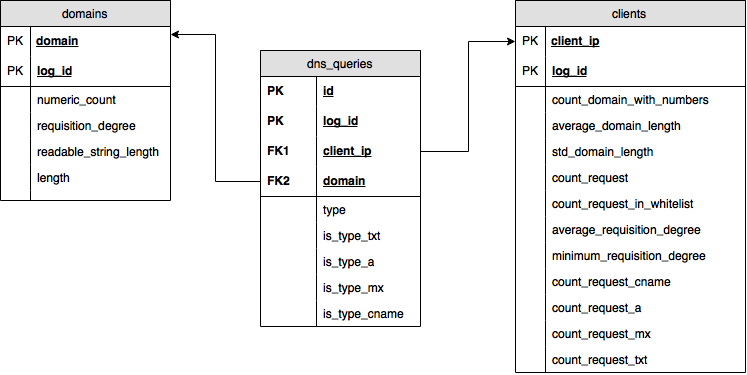
\includegraphics[width=\textwidth]{relational_diagram}
\caption[Diagrama Relacional do Sistema]{Diagrama Relacional do Sistema} \label{fig:relational_diagram}
\end{figure}

A tabela \textit{dns\_queries} é a que melhor representa a estrutura bruta do log de DNS. Mesmo sendo simples, sem muitos tratamentos, ela já apresenta consultas interessantes, como verificar que domínios uma máquina consultou. Os campos \textit{is\_type\_a}, \textit{is\_type\_mx}, \textit{is\_type\_cname}, \textit{is\_type\_txt} são booleanos e indicam apenas se o domínio é do tipo especificado. Embora essa informação já esteja presente na coluna \textit{type}, eles foram adicionados para facilitar cálculos posteriores. A Figura \ref{fig:dns_queries} mostra exemplos de algumas entradas nessa tabela, o cálculo da coluna \textit{query\_time} ainda não foi implementado.

\begin{figure}
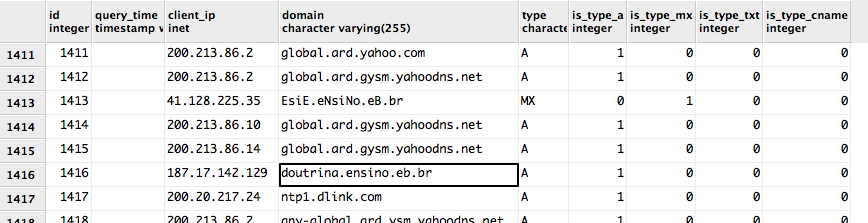
\includegraphics[width=\textwidth]{dns_queries}
\caption[Exemplos de entradas na tabela \textit{dns\_queries}]{Exemplos de entradas na tabela \textit{dns\_queries}} \label{fig:dns_queries}
\end{figure}

A tabela \textit{domains} contém informações referentes à cada domínio consultado. A coluna \textit{length} representa a quantidade de caracteres presentes no nome do domínio. A coluna \textit{numeric\_count} contém a informação de quantos caracteres numéricos estão presentes no domínio. A coluna \textit{readable\_string\_length} calcula a maior \textit{substring} legível do domínio, porém essa coluna não foi utilizada posteriormente, já que o ideal seria calcular o tamanho total legível da \textit{string}, mas devido a complexidade desse cálculo  ele não foi utilizado. A coluna \textit{is\_in\_whitelist} verifica se o domínio está na \textit{whitelist} utilizada, porém verificou-se que muitos domínios consultados conhecidos não estavam lá, abrindo margem para aprimoramento ao incrementar a \textit{whitelist} utilizada para o cenário do Exército Brasileiro. Finalmente, a coluna \textit{requisition\_degree} é bem interessante, informando o grau de requisição do domínio, ou seja, quantas máquinas diferentes também consultaram esse domínio. A Figura \ref{fig:domains} mostra exemplos de algumas entradas nessa tabela, o cálculo das colunas \textit{is\_suspect} e \textit{alexa\_degree} ainda não foi implementado.

\begin{figure}
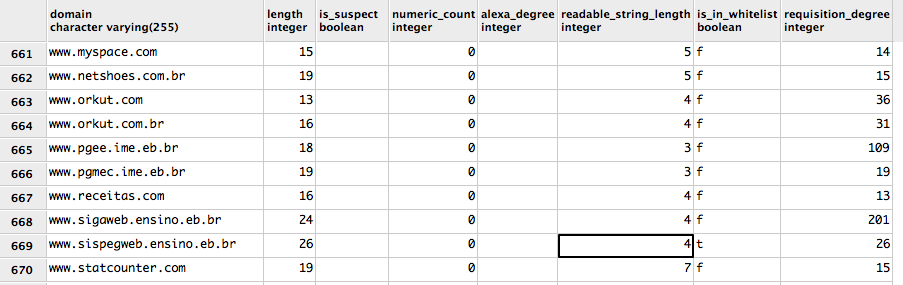
\includegraphics[width=\textwidth]{domains}
\caption[Exemplos de entradas na tabela \textit{domains}]{Exemplos de entradas na tabela \textit{domains}} \label{fig:domains}
\end{figure}

A tabela \textit{clients} representa as máquinas que fizeram requisições DNS no período de tempo analisado, sendo assim, ela é a mais importante para os algoritmos de aprendizado, já que o sistema está preocupado em descobrir as máquinas infectadas. O cálculo das colunas é feito com o auxílio das tabelas \textit{domains} e \textit{dns\_queries}, que guardam a informação de como o cliente tem se comportado na rede. Suas colunas são basicamente as características que são analisadas na seção seguinte. Na figura \ref{fig:clients} são mostrados alguns valores para essas colunas. Devido ao elevado número de colunas nessa tabela, algumas delas foram omitidas para melhorar a visualização.

\begin{figure}
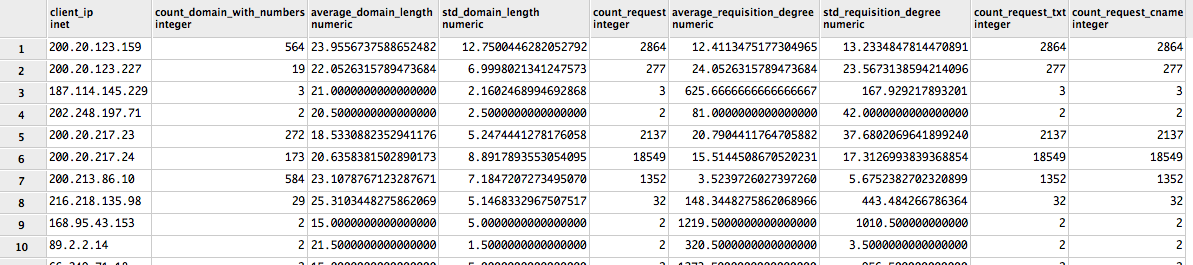
\includegraphics[width=\textwidth]{clients}
\caption[Exemplos de entradas na tabela \textit{clients}]{Exemplos de entradas na tabela \textit{clients}} \label{fig:clients}
\end{figure}

\section{Levantamento das Características}
De posse das informações apresentadas nos capítulos anteriores, é possível definir mais claramente o problema que esse trabalho se propõe a resolver e, em linhas gerais, como ele será abordado.

O objetivo desse trabalho é a partir das informações obtidas no log de registros de um servidor DNS, acusar quais máquinas na rede são suspeitas de pertencer a uma botnet e merecem atenção para uma investigação mais profunda. Para isso, foram pensadas características que uma máquina pertencente a uma botnet pode exibir que a distingue de uma máquina com uso normal.

As características analisadas foram divididas em quatro tipos, que identificam comportamentos divergentes do uso comum que esperam ser observados: a forma de escolha dos domínios, o comportamento de máquina, os domínios visitados em comum e tipos de requisição.

\subsection{Escolha dos Domínios}
Muitas botnets utilizam técnicas de geração de domínio \citep{zhou2013dga}. Essa técnica permite que os bots consultem um grande conjunto de domínios a procura do C\&C, porém apenas um pequeno conjunto desses domínios são de fato utilizados. Essa prática gera nomes não legíveis, muitas vezes formados apenas por números e palavras não legíveis. Além disso, por conveniência, é possível que os domínios gerados por uma mesma botnet tenham o mesmo número de caracteres. Por outro lado, apenas 7.3\% dos domínios dos um milhão primeiros domínios da Alexa contem número e que o tamanho do domínio de um usuário comum não segue nenhum padrão específico.

Não há garantia que essa feature é sempre efetiva, dado que o atacante pode gerar domínios de tamanho variável e evitar números ao gerar o domínio, por isso após a realização dos experimentos será possível confirmar ou não essa hipótese.

Para explorar essas propriedades foram propostas as seguintes características 

\begin{itemize}
\item Quantidade de consultas a domínios com números 
\item Média do comprimento de domínios consultados
\item Desvio Padrão dos comprimentos dos domínios consultados
\end{itemize}

\subsection{Comportamento de Máquina}

O tempo de reação de um humano a uma requisição sem sucesso não pode ser de décimos de segundo, por mera limitação de reflexo. Qualquer sinal de uso que apresente um baixo intervalo entre consultas, algo que apenas uma máquina pode fazer, deve ser considerada suspeita. Além disso, é possível que a máquina acabe por visitar uma quantidade de domínios maior do que o normal ou faça consultas em intervalos regulares, pré-programados, coisa que um ser humano normal raramente irá realizar. Novamente, esse tipo de feature precisa ser validado, pois o comportamento de máquina pode ser mascarado, ao configurar um intervalo aleatório entre consultas e com um certo atraso.

Para explorar essas propriedades foram propostas as seguintes características 

\begin{itemize}
\item Média do intervalo entre as consultas
\item Desvio padrão dos intervalos entre consultas
\item Quantidade total de consultas realizadas
\end{itemize}

\subsection{Domínio Visitados em Comum}
Espera-se que domínios suspeitos sejam acessados apenas por poucas máquinas, como os domínios gerados por algoritmos de geração de domínios para tentar estabelecer uma comunicação com o C\&C. Devido a isso, espera-se que os bots tentem acessar domínios que dificilmente serão procurados por máquinas normais, além do que, se a máquina infectada procura o centro de comando e controle, espera-se que muito dos domínios consultados por ela também sejam dessa forma, ou seja pouco procurado por outras máquinas.

Para analisar essa propriedade, foi necessário realizar um pré-processamento, que analisa para cada domínio consultado, por quantas máquinas diferentes ele foi consultado. Essa quantidade de máquinas que requisitou um domínio específico chamaremos de grau de requisição do domínio.

Dessa forma, acredita-se que as informações relativas ao grau dos domínios consultados pela máquina podem ser úteis para identificar um comportamento suspeito em uma máquina. Foram levantadas as seguintes características:

\begin{itemize}
\item Grau de requisição mínimo entre os graus dos domínios consultados pela máquina
\item Média dos graus de requisição dos domínios consultados pela máquina
\item Desvio Padrão dos graus de requisição dos domínios consultados pela máquina

\end{itemize}

\subsection{Tipos de Requisição}

Não se tem informação sobre máquinas seguindo padrão quanto ao tipo de requisição DNS solicitadas. Porém, esse dado é de fácil acesso e seu estudo pode evidenciar a exploração de alguma fragilidade ainda não analisada nas requisições DNS. Por exemplo, os registros do tipo TXT raramente são utilizados atualmente para leitura de seres humanos. Para isso levantamos algumas características quanto ao tipos de requisição DNS realizadas:

\begin{itemize}
\item Quantidade de consultas do tipo A (Registro de Endereço) realizadas
\item Porcentagem de consultas do tipo A realizadas
\item Quantidade de consultas do tipo MX (Registro de Troca de Mensagens) realizadas
\item Porcentagem de consultas do tipo MX realizadas
\item Quantidade de consultas do tipo CNAME (Nome Canônico) realizadas
\item Porcentagem de consultas do tipo CNAME realizadas
\item Quantidade de consultas do tipo TXT (Registro de Texto) realizadas
\item Porcentagem de consultas do tipo TXT realizadas
\end{itemize}

Com essas informações calculadas, é possível submeter as informações contidas no log de DNS para serem tratadas por algoritmos de agrupamento. Espera-se que os bots apresentem comportamento diferente de usuários normais, seguindo padrões que não são seguidos por usuários normais, fazendo com que eles fiquem agrupados em grupos menores, que devem ser investigados.

\chapter{Resultados e Discussões}\label{ch:discussion}

Os experimentos foram realizados com a base de dados organizada como descrita no Capítulo 4 relativo à Preparação de Dados. Os experimentos foram feitos com o apoio da ferramenta \textit{Scikit-Learn} que possui a implementação de diversos algoritmos de aprendizado de máquina e agrupamento, dentre eles K-Médias, que já foi discutido no capítulo 3. Também foi utilizado o pacote \textit{NumPy}, ferramenta para cálculos matriciais não menos importantes para o sucesso do trabalho.

Para a preparação das análises foi adicionado ao banco de dados o registro de atividades do servidor DNS do IME de 12 de março de 2012. Nesse registro de atividades há rastros de 3 suspeitos já confirmados como parte integrante de botnets, através de inspeções manuais feitas na época.

Foi realizada a comparação da qualidade da saída algoritmo para dados normalizados e não normalizados. Para normalizar, decidiu-se arbitrariamente, utilizar a forma \ref{eq:norm}

\begin{equation} \label{eq:norm}
\frac{\mathbf{X} - \mathbf{\bar{X}}}{\sigma}
\end{equation}

\section{Análise do Número de Grupos}

Para o cálculo da distribuição da função custo, foram criados 10 modelos para cada quantidade de centroides e calculou-se a média das funções de custos dentre cada quantidade de centroide. Esse procedimento é realizado para estabilizar os valores da função custo, já que a função custo pode estar sujeita a flutuação, por outro lado isso não pareceu crítico para esse conjunto de dados.

As figuras \ref{fig:cost_per_k} e \ref{fig:cost_per_k_not_norm} apresentam o comportamento dos valores da função custo ao serem adicionados centroides.

\begin{figure}[htbp]
\centering
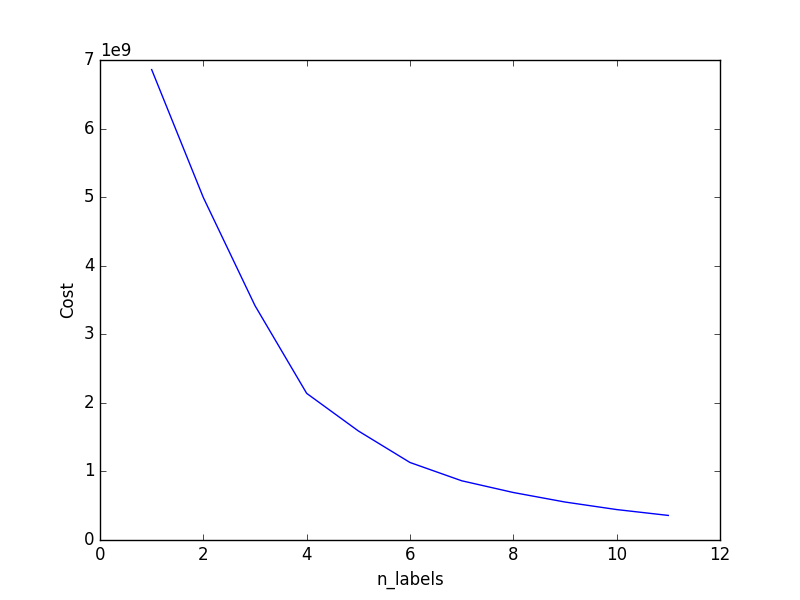
\includegraphics[scale=0.7]{cost_per_k}
\caption[Custo pelo Número de Centroides para Dados Normalizados]{Custo pelo Número de Centroides para Dados Normalizados} \label{fig:cost_per_k}
\end{figure}

\begin{figure}[htbp]
\centering
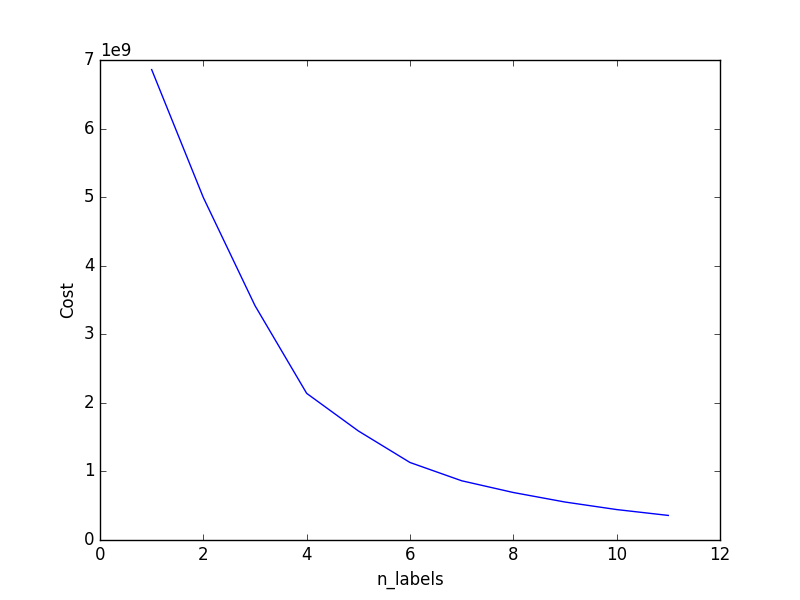
\includegraphics[scale=0.7]{cost_per_k_not_norm}
\caption[Custo pelo Número de Centroides para Dados não Normalizados]{Custo pelo Número de Centroides para Dados não Normalizados} \label{fig:cost_per_k_not_norm}
\end{figure}

Apesar de se perceber um bico quando o modelo tem 4 centroides em ambas figuras, ainda há ambiguidade quanto ao ponto crítico. Outras técnicas mais robustas serão avaliadas nas fases posteriores do projeto para validar a hipótese de que há utilização de 4 centroides gera os melhores resultados.

\section{Análise da Base de Dados}

Utilizando-se 4 centroides como parâmetro, foram realizadas análises da eficácia do algortimo de agrupamento ao conjunto de exemplos contidos no banco de dados. Em todos os experimentos o sistema consulta a tabela \textit{clients} do banco de dados e retorna na saída padrão a cardinalidade de cada grupo e os IPs das máquina no menor grupo.

A primeira análise foi realizada observando os seguintes campos:

\begin{itemize}
\item \textit{count\_domain\_with\_numbers, }
\item \textit{average\_domain\_length, }
\item \textit{std\_domain\_length, }
\item \textit{count\_request, }
\item \textit{average\_requisition\_degree, }
\item \textit{std\_requisition\_degree e }
\item \textit{minimum\_requisition\_degree }
\end{itemize}

Os dados foram fornecidos ao algoritmo sem nenhum tratamento posterior, já que os dados já foram tratados previamente. Como resultado obteve-se a saída representada na figura \ref{fig:first_out}. Esse resultado não foi considerado um sucesso, pois o menor grupo não continha nenhum dos 3 suspeitos conhecidos, porém já apresenta um grupo de cardinalidade reduzida conforme era esperado.

\begin{figure}[htbp]
\centering
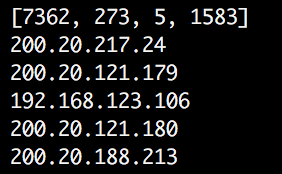
\includegraphics[scale=0.7]{first_out}
\caption[Resultado do Experimento não Normalizado]{Resultado do Experimento não Normalizado} \label{fig:first_out}
\end{figure}

Para a segunda análise, foi efetuada a normalização das características, para que cada uma tivesse o mesmo impacto para as distâncias utilizadas no algoritmo, independente do intervalo para os valores de cada uma. Após essa alteração, observou-se a saída mostrada na Figura \ref{fig:second_out}. Esse foi considerado um resultado bastante satisfatório, já que duas máquinas já confirmadas como pertencentes a botnets foram detectadas no menor grupo, cujos endereços de IP são \textit{200.213.86.2} e \textit{200.213.86.14}.

\begin{figure}[htbp]
\centering
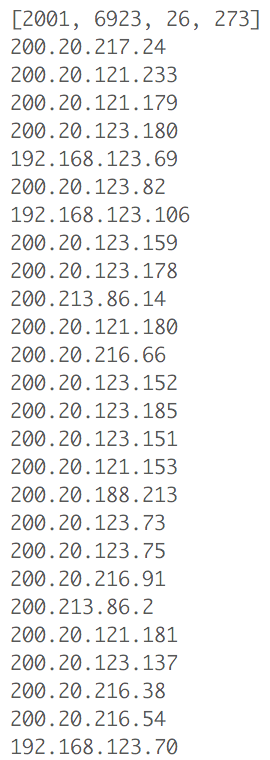
\includegraphics[scale=0.7]{second_out}
\caption[Resultado do Experimento Normalizado]{Resultado do Experimento Normalizado} \label{fig:second_out}
\end{figure}

A hipótese que se levanta para explicar o sucesso é que apesar de as máquinas com comportamento suspeito divergirem das outras máquinas, por exemplo em quantidade de requisição, a distância marginal entre elas é grande o suficiente para confundir o algoritmo ao tentar agrupa-los.

Além disso observou-se que, ao ser descartado, o campo \textit{std\_requisition\_degree} não influenciou na identificação dos itens do menor grupo, isto é os mesmo 26 elementos permanecem consistentemente no mesmo grupos. Isso reforça a necessidade de ser aplicada uma técnica para realizar a seleção das melhores características.
\chapter{A Ferramenta de Detecção}
A ferramenta para detecção de botnets foi desenvolvida utilizando o Ambiente de Desenvolvimento Integrado (\textit{Integrated Development Environment} - IDE) \textit{Qt Creator}. A tela inicial do sistema pode ser vista na Figura \ref{fig:initial_screen}.

\begin{figure}
\centering
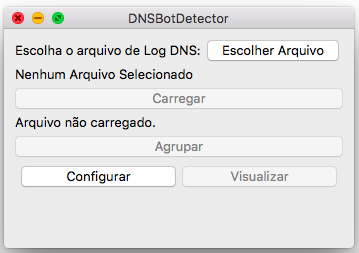
\includegraphics[width=10cm]{initial_screen}
\caption[Tela inicial da Ferramenta]{Tela inicial da Ferramenta} \label{fig:initial_screen}
\end{figure}

Qt é um IDE multi-plataforma que permite desenvolver aplicações com interface gráfica utilizando a linguagem C++ \citep{qtsite}. A escolha de Qt para o desenvolvimento da plataforma foi motivada pelo fato dele ser multi-plataforma, assim como o banco de dados utilizado (PostgreSQL), além do suporte à C++, que foi a linguagem adotada na fase inicial para implementar a preparação de dados.

A aplicação desenvolvida no Qt se comunica com o módulo desenvolvido em Python que serve de interface para leitura do banco de dados até o consumo final dos dados do banco, seja através de planilhas ou gráficos de distribuição espacial. As transações entre o interface gráfica e Python foram todas feitas através de criação de processos paralelos.

Ao longo dessa seção é exibida a documentação das funcionalidades do sistema, além de uma visão geral sobre a aplicação desenvolvida.

\section{Documentação de Casos de Uso}
Nesta seção é mostrada a documentação dos casos de usos atendidos pelo sistema. São 5 casos de uso no total: Carregar Arquivo de Log DNS (Tabela \ref{tab:use_case_load_file}), Configurar Técnica de Agrupamento (Tabela \ref{tab:use_case_config}), Visualizar Gráfico (Tabela \ref{tab:use_case_visualize}), Realizar Agrupamento (Tabela \ref{tab:use_case_clustering}) e Identificar Cliente no Gráfico (Tabela \ref{tab:use_case_identify}). O diagrama dos casos de usos pode ser visto na Figura \ref{fig:diagram_use_cases}. 

\begin{figure}
\centering
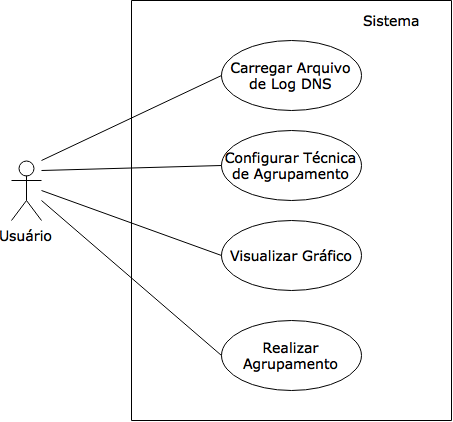
\includegraphics[width=12cm]{diagram_use_cases}
\caption[Diagrama de Casos de Uso]{Diagrama de Casos de Uso} \label{fig:diagram_use_cases}
\end{figure}

A descrição de cada caso de uso é feita em tabelas para melhor visualização. Essas descrições podem então ser vistas nas tabelas dessa seção. 

No modelo de especificação de casos de uso utilizado, os passos do Fluxo Básico de Eventos (FBE), são referenciados no Fluxo Alternativo de Eventos. Além disso, as pós-condições são atendidas quando o caso de uso é encerrado com sucesso. Nos casos de falha, a não ser que algo seja especificado, o sistema retorna ao estado em que estava antes do caso de uso ter sido iniciado.

\begin{table}[]
\centering
\caption{Caso de Uso - Carregar Arquivo de Log DNS}
\label{tab:use_case_load_file}
\begin{tabular}{|lp{10cm}|}
\hline
Nome: & Carregar Arquivo de Log DNS  \\ \hline
Ator: & Usuário   \\ \hline
Pré-condições: & Nenhuma   \\ \hline
\multirow{15}{*}{Fluxo Básico de Eventos:} & 1. O Usuário seleciona a opção ``Escolher Arquivo''  \\
 & 2. O Sistema exibe uma janela com os arquivos no formato txt presentes no sistema de arquivos do Usuário.  \\
 & 3. O Usuário seleciona um arquivo de log para importar.  \\
 & 4. O Sistema informa o endereço do arquivo selecionado e disponibiliza a opção ``Carregar''. \\
 & 5. O Usuário seleciona a opção ``Carregar'' \\
 & 6. O Sistema exibe um \textit{pop-up} informando que o arquivo está sendo importado para o banco de dados e inicializa a importação dos dados do arquivo para o banco de dados. \\
 & 7. O Sistema retira o \textit{pop-up} informando que o arquivo está sendo importado para o banco de dados e altera a mensagem ``Arquivo não carregado'' para ``Arquivo de Logs Carregado com Sucesso!'' e o caso de uso é encerrado com sucesso.\\ \hline
\multirow{3}{*}{Fluxo Alternativo de Eventos:} & \textbf{(A1) Nenhum Arquivo Selecionado:} No passo 4 do FBE se nenhum arquivo tiver sido selecionado.\\
 & A1.a) O caso de uso é encerrado com falha.\\ \hline
\multirow{5}{*}{Pós-Condições:} & 1. Os dados contidos no log informado pelo usuário foram carregados no banco de dados. \\
 & 2. As opções ``Agrupar'' e ``Visualizar'' são disponibilizadas.\\
 & 3. A opção ``Carregar'' é desativada.\\
\hline 
\end{tabular}
\end{table}

\begin{table}[]
\centering
\caption{Caso de Uso - Configurar Técnica de Agrupamento}
\label{tab:use_case_config}
\begin{tabular}{|lp{10cm}|}
\hline
Nome: & Configurar Técnica de Agrupamento  \\ \hline
Ator: & Usuário   \\ \hline
Pré-condições: & Nenhuma   \\ \hline
\multirow{12}{*}{Fluxo Básico de Eventos:} & 1. O Usuário seleciona a opção ``Configurar''  \\
 & 2. O Sistema recupera as informações do último arquivo de configuração salvo. \\
 & 3. O Sistema exibe as opções disponíveis para as Informações de Configuração, pré-selecionando as opções recuperadas no passo 2. \\
 & 4. O Usuário seleciona as Informações de Configuração desejadas.  \\
 & 5. O Sistema exclui o arquivo de configuração anterior, salva as Informações de Configuração selecionadas pelo Usuário em um novo arquivo de configuração e o caso de uso é encerrado com sucesso. \\
 \hline
\multirow{9}{*}{Fluxo Alternativo de Eventos:} & \textbf{(A1) Arquivo de Configuração Não Encontrado:} No passo 2 do FBE se o Sistema detectar que o arquivo de configuração anterior não existe.\\
 & A1.a) O Sistema utiliza os valores padrões como informação recuperada do arquivo.\\
 & A1.b) O Sistema retorna ao passo 3 do FBE. \\ 
 & \textbf{(A2) Janela de Configuração Cancelada:} No passo 5 do FBE se o Usuário cancelar a janela de configuração. \\
 & A2.a) O caso de uso é encerrado com falha. \\
 \hline
\multirow{2}{*}{Pós-Condições:} & 1. As Informações de Configuração selecionadas pelo Usuário são armazenadas no arquivo de configuração. \\
\hline
\multirow{10}{*}{Outras Informações:} & 1. Informações de Configuração: Lista de Características para Agrupamento, Algoritmo de Agrupamento e Número de Grupos. \\
 & 2. Valores Padrão: Lista de Características para Agrupamento: [\textit{count\_domain\_with\_numbers, average\_domain\_length, std\_domain\_length, count\_request, average\_requisition\_degree, std\_requisition\_degree, minimum\_requisition\_degree}], Algoritmo de Agrupamento: K-Médias, Número de Grupos: 4. \\
\hline 
\end{tabular}
\end{table}

\begin{table}[]
\centering
\caption{Caso de Uso - Visualizar Gráfico}
\label{tab:use_case_visualize}
\begin{tabular}{|lp{10cm}|}
\hline
Nome: & Visualizar Gráfico  \\ \hline
Ator: & Usuário   \\ \hline
\multirow{2}{*}{Pré-Condições:} & Os dados contidos no log DNS foram carregados no banco de dados.  \\ \hline
\multirow{10}{*}{Fluxo Básico de Eventos:} & 1. O Usuário seleciona a opção ``Visualizar''  \\
 & 2. O Sistema exibe a Lista de Características para Agrupamento disponíveis para serem visualizadas. \\
 & 3. O Usuário seleciona 2 ou 3 características que deseja visualizar em um gráfico e seleciona a opção ``cria gráfico''. \\
 & 4. O Sistema buscará no banco de dados pelos endereços IP e as características selecionadas e apresenta os pontos resultantes em um gráfico e o caso de uso termina com sucesso  \\
 \hline
\multirow{5}{*}{Fluxo Alternativo de Eventos:} & \textbf{(A1) Quantidade de características inválida:} No passo 3 do FBE se o cliente selecionar qualquer quantidade abaixo de 2 e acima de 3.\\
 & A1.a) O Sistema exibe uma mensagem de erro e o caso de uso termina com falha.\\
 \hline
\multirow{2}{*}{Pós-Condições:} & 1. O Sistema exibiu o gráfico interativo com os eixos informados pelo Usuário. \\
\hline
\multirow{5}{*}{Outras Informações:} & 1. Lista de Características para Agrupamento: [\textit{count\_domain\_with\_numbers, average\_domain\_length, std\_domain\_length, count\_request, average\_requisition\_degree, std\_requisition\_degree, minimum\_requisition\_degree}].  \\
\hline 
\end{tabular}
\end{table}

\begin{table}[]
\centering
\caption{Caso de Uso - Realizar Agrupamento}
\label{tab:use_case_clustering}
\begin{tabular}{|lp{10cm}|}
\hline
Nome: & Realizar Agrupamento  \\ \hline
Ator: & Usuário   \\ \hline
\multirow{2}{*}{Pré-Condições:} & Os dados contidos no log DNS foram carregados no banco de dados.  \\ \hline
\multirow{12}{*}{Fluxo Básico de Eventos:} & 1. O Usuário seleciona a opção ``Agrupar''  \\
 & 2. O Sistema apresenta um ambiente para a escolha do destino do arquivo. \\
 & 3. O Usuário escolhe a pasta onde será salvo e o nome do arquivo. \\
 & 4. O Sistema agrupa os IPs segundo suas características resgatadas no banco de dados e aplica um algoritmo de agrupamento com parâmetros definidos no arquivo de configuração.  \\
 & 5. O Sistema salva os IPs e suas características na pasta escolhida pelo usuário e o caso de uso termina com sucesso. \\
 \hline
\multirow{3}{*}{Pós-Condições:} & 1. O arquivo no formato XLS é armazenado no endereço definido pelo Usuário com as informações de cada grupo separadas por aba. \\
\hline
\end{tabular}
\end{table}

\begin{table}[]
\centering
\caption{Caso de Uso - Identificar Cliente no Gráfico}
\label{tab:use_case_identify}
\begin{tabular}{|lp{10cm}|}
\hline
Nome: & Identificar Cliente no Gráfico  \\ \hline
Ator: & Usuário   \\ \hline
\multirow{2}{*}{Pré-Condições:} & O Sistema exibiu o gráfico interativo com os eixos informados pelo Usuário.  \\ \hline
\multirow{6}{*}{Fluxo Básico de Eventos:} & 1. O Usuário seleciona o ponto no gráfico que deseja identificar.  \\
 & 2. O Sistema recupera as informações do ponto, exibe em um rótulo no gráfico interativo o endereço de IP da máquina cliente no ponto desejado e o caso de uso termina com sucesso. \\
 \hline
 \multirow{2}{*}{Pós-Condições:} & 1. O Sistema exibiu o endereço de IP da máquina que estava no ponto selecionado. \\
 \hline
\end{tabular}
\end{table}

\section{Visão Geral do Sistema}
A aplicação desenvolvida serve para auxiliar na detecção de botnets. Esse auxílio é feito baseado em informações coletadas por um servidor de DNS. Para oferecer informações relevantes ao usuário, utilizando os algoritmos de agrupamento, a aplicação segue um fluxo básico, constituídos por etapas distintas: Leitura do Log DNS, Cálculo das Informações dos Domínios, Cálculo das Características das Máquinas, Seleção das Configurações, Execução do Algoritmo de Agrupamento e Disponibilização dos Resultados no Arquivo XLS. A Figura \ref{fig:program_flow} mostra um diagrama do fluxo básico de funcionamento do sistema.

\begin{figure}
\centering
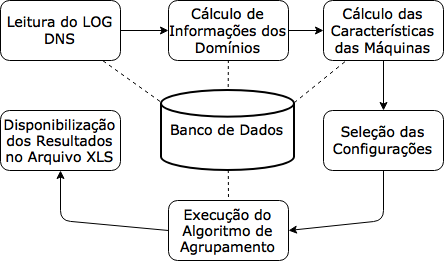
\includegraphics[width=12cm]{program_flow}
\caption[Diagram do Fluxo do Programa]{Diagrama do Fluxo do Programa} \label{fig:program_flow}
\end{figure}

As primeiras etapas que devem ser cumpridas, são as seguintes: Leitura de Log DNS, Cálculo das Informações das Informações dos Domínios e Cálculo das Características que são concluídas durante o caso de uso descrito na Tabela \ref{tab:use_case_load_file}. Na etapa de Leitura de Log DNS, é feita a extração das informações brutas coletadas pelo servidor DNS para o banco de dados. Nas etapas de Cálculo, as informações são calculadas utilizando chamadas as funções de agrupamento do SQL. A Figura \ref{fig:screen_file_loaded} mostra o estado da aplicação após a conclusão do caso de uso Carregar Arquivo de Log DNS, onde pode ser visto que a aplicação libera a utilização das opções ``Agrupar'' e ``Visualizar''.

\begin{figure}
\centering
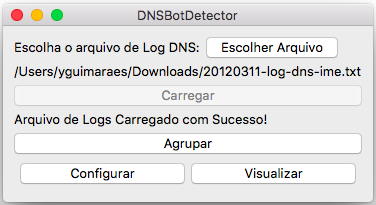
\includegraphics[width=10cm]{screen_file_loaded}
\caption[Tela do Sistema após Executar o Caso de Uso Carregar Arquivo de Log DNS]{Tela do Sistema após Executar o Caso de Uso Carregar Arquivo de Log DNS} \label{fig:screen_file_loaded}
\end{figure}

A Etapa de Seleção das Configurações, descrita pelo caso de uso na Tabela \ref{tab:use_case_config} é opcional, pois caso não seja realizada a aplicação carregará os valores padrão ou os utilizados em outro uso prévio da ferramenta. Essa etapa serve para que o usuário escolha as características que deseje que o algoritmo de agrupamento utilize, especifique o algoritmo de agrupamento desejado e o número de grupos que devem ser formados. A Figura \ref{fig:screen_config} mostra a tela na qual o usuário pode realizar essas configurações.

\begin{figure}
\centering
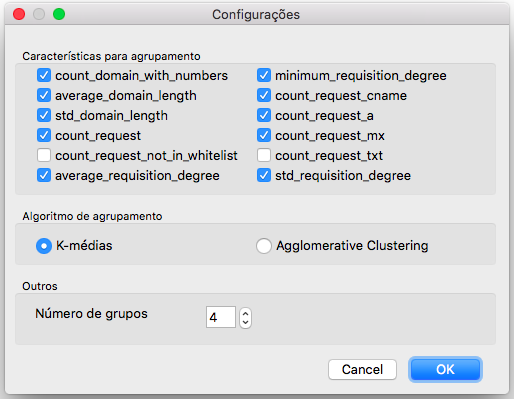
\includegraphics[width=10cm]{screen_config}
\caption[Tela do Sistema para Realizar a Seleção das Configurações]{Tela do Sistema para Realizar a Seleção das Configurações} \label{fig:screen_config}
\end{figure}

Por fim, as etapas de Execução do Algoritmo de Agrupamento e Disponibilização dos Resultados no Arquivo XLS acontecem na execução do caso de uso na Tabela \ref{tab:use_case_clustering}. Nesse etapa, o algoritmo de agrupamento escolhido é executado com os parâmetros selecionados na Etapa de Seleção das Configurações para as máquinas que estavam presentes no arquivo de log DNS utilizado. Em seguida, os resultados do algoritmo de agrupamento são persistidos no arquivo XLS com nome e caminho definidos pelo usuário da aplicação. Nesse arquivo, cada aba representa um grupo que foi identificado pelo algoritmo e contém as máquinas presentes nos respectivos grupos. A Figura \ref{fig:screen_xls_file} mostra a visualização desse arquivo.

\begin{figure}
\centering
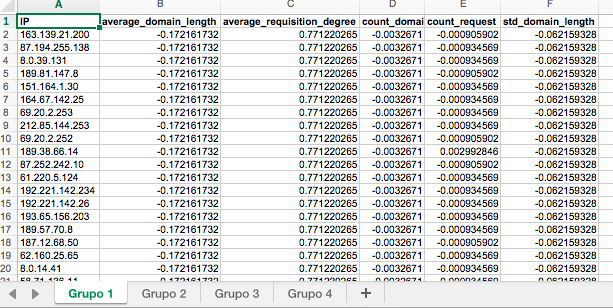
\includegraphics[width=13cm]{screen_xls_file}
\caption[\textit{Layout} do Arquivo XLS Gerado com os Resultados do Agrupamento]{\textit{Layout} do Arquivo XLS Gerado com os Resultados do Agrupamento} \label{fig:screen_xls_file}
\end{figure}

\begin{figure}
\centering
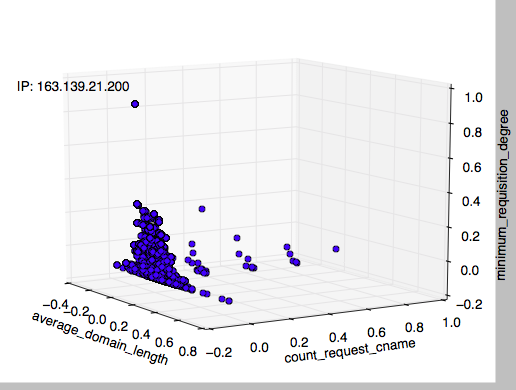
\includegraphics[width=12cm]{3d_graf_example}
\caption[\textit{Layout}  do Gráfico Gerado com um Ponto Isolado Selecionado]{\textit{Layout}  do Gráfico Gerado com um Ponto Isolado Selecionado} \label{fig:3d_graf_example}
\end{figure}

A aplicação apresenta também a funcionalidade de geração de gráficos. Uma funcionalidade da aplicação se encontra fora do fluxo principal da técnica de inteligência artificial, mas se mostrou preciosa para auxiliar na seleção das melhores características, além de permitir encontrar máquinas suspeitas visualmente. Os casos de uso dessa parte se encontram descritos nas tabelas \ref{tab:use_case_visualize} e \ref{tab:use_case_identify}.

Esses gráficos permitem identificar como as máquinas estão distribuídas espacialmente de acordo com as características selecionadas. Ou seja, o usuário pode selecionar 2 ou 3 características e visualizar o gráfico de como elas se encontram distribuídas no espaço. Isso permite identificar se as características utilizadas são úteis, ao exibir como a distribuição das máquinas se comporta com os valores de características selecionadas. Além disso, o usuário pode identificar os endereços de IP dos pontos que estão muito fora da normalidade, como na Figura \ref{fig:3d_graf_example} comportamento que pode ser considerado suspeito, auxiliando na detecção mais uma vez.

%\chapter{Cronograma}
Embora o objetivo do trabalho seja o desenvolvimento de um projeto e não pesquisa, foi preciso começar por um intenso estudo do problema que queríamos resolver, ou seja das botnets. Isso é uma etapa importante de um projeto de aprendizagem de máquina, pois permite uma melhor identificação de quais features serão mais relevantes.

Em seguida, foi feito um estudo dos algoritmos de clustering existentes e os objetivos de cada técnica.

Após esses estudos, começa a implementação do sistema detector de botnets. A primeira etapa é desenvolver um tratamento automatizado dos dados obtidos pela coleta dos logs DNS, já que o objetivo final é de que esse tratamento seja feito diariamente. Depois serão implementados algoritmos de agrupamento que usarão os dados tratados para identificar padrões de botnets no log DNS coletado. Por fim, os resultados dessas técnicas serão testados e analisados e servirão de motivação para possíveis refinamentos nos algoritmos.

Durante essas tarefas, desenvolveremos também os relatórios e apresentações para as seguintes avaliações:

\begin{itemize}  
\item Verificação Especial em Maio,
\item Verificação Corrente em Julho,
\item Verificação Final em Setembro.
\end{itemize}

\begin{landscape}
\begin{figure}
\centering
\begin{ganttchart}[
	hgrid,
	vgrid,
	x unit=1.8cm,
	compress calendar,
    bar/.append style={fill=green!40},
	time slot format=isodate-yearmonth
]{2016-02}{2016-09}
\gantttitlecalendar{year, month=shortname} \\
\ganttbar{Estudo de Botnets}{2016-02}{2016-02} \\
\ganttbar{Estudo de Clustering}{2016-02}{2016-03} \\
\ganttbar{Escolha das possíveis features}{2016-02}{2016-03} \\
\ganttbar{Preparação dos Dados}{2016-03}{2016-04} \\
\ganttbar{Preparar Relatório e Apresentação VE}{2016-04}{2016-05} \\
\ganttbar{Selecionar e Implementar Algoritmos de Clustering}{2016-06}{2016-07} \\
\ganttbar{Preparar Relatório e Apresentação VC}{2016-07}{2016-07} \\
\ganttbar{Teste e Análise de Resultados}{2016-08}{2016-09} \\
\ganttbar{Refinar Algoritmos}{2016-08}{2016-09} \\
\ganttbar{Preparar Relatório e Apresentação VF}{2016-09}{2016-09} \\
\end{ganttchart}
\caption[Cronograma]{Cronograma} \label{fig:cronograma}
\end{figure}
\end{landscape}
\chapter{Conclusão}

Os clientes IP foram modeladas segundo algoritmos de agrupamento apresentados no Capítulo \ref{ch:machine} utilizando características levantadas no Capítulo \ref{ch:data_preparation}. Essas caracterísiticas evidenciam os bots se considerando a arquitetura das botnets estudada no Capítulo \ref{ch:botnet}. Dessa forma foi desenvolvido uma ferramenta de apoio à decisão na detecção de bots em log DNS a qual as especificações do caso de uso e as janelas de diálogo foram apresentadas no Capítulo \ref{ch:tool}

A primeira contribuição evidente do trabalho foi próprio desenvolvimento da ferramenta de apoio a decisão que reduz o domínio de análise do usuário através dos algoritmos de agrupamento e permite a visualização dos dados seguindo nos eixos as características previamente levantadas como relevante

Além disso, como contribuição de conhecimento pode-se ressaltar a análise da variação da função custo do modelo gerado pelo K-Médias a cada centroide adicionado ao modelo. Percebeu-se que o Método \textit{Elbow} não é satisfatório para essa análise.

Como alternativa para a descoberta da quantidade centroides foi implementada uma solução de visualização dos dados que permite resgatar as informações de cada ponto escolhido. Essa solução ainda não se mostrou a melhor quando aplicada na base de dados conhecida, mas se mostrou muito útil também para detectar pontos que fogem do padrão mais comum.

Foi feita uma análise no log DNS do IME de 12 de março de 2012 e foi alcançado um resultado satisfatório no qual duas das três máquinas suspeitas já conhecidas estavam presentes no menor grupo.

Como já salientado, a complexidade do algoritmo de Agrupamento por Aglomeração é alta, por isso é importante manter um \textit{cache} dos resultados computados pelo algoritmo para que a troca da quantidade de grupos não apresente a demora de uma primeira contrução da hierarquia dos grupos.

Após uma breve comparação dos dados normalizados contra os não-normalizados, percebeu-se o esperado, é melhor trabalhar com dados normalizados. O resultado era esperado pois, algumas características geram números de ordem muito maior do que a maioria e ainda apresentavam grandes diferenças entre si. Para o algoritmo corria-se o risco haver grupos separados por essa distância relativa.

Apesar desse trabalho ter realizado uma análise, o que inclusive foge um pouco do escopo do projeto, espera-se que em trabalhos futuros as análises com outros dados sejam realizadas. Além disso, espera-se um estudo qualitativo das características implementadas um bom trabalho para o log DNS utilizado, mas não necessariamente se comportará bem com todo tipo de fluxo no log DNS. Espera-se também que seja estudado o algoritmo de agrupamento aglomerativo, o qual foi integrado ao trabalho mas não foi teve resultados analisados. Outros algoritmos devem ser analisados, para validar a solução e garantir o pleno apoio à decisão que esse trabalho se propõe.

% -----
% PARTE DE REFERÊCIAS BIBLIOGRÁFICAS DE PFC
%
%  As referências do documento de PFC devem estar no arquivo refs.bib
%  Devem seguir o formato bibtex - ver Manual-Referencias.pdf para mais detalhes.
% -----
\bibliographystyle{pfc}
\bibliography{refs}

% -----
% PARTE DE APÊNDICE DE PFC
%
%  Se o documento de PFC não tiver apêndices REMOVER AS LINHAS ABAIXO
%  Adicionar os arquivos .tex de apêndice ao documento com comando \include{•}
% -----
%\inappendix
%%%
%
% ARQUIVO: apendice.tex
%
% VERSÃO: 1.0
% DATA: Maio de 2016
% AUTOR: Coordenação de Trabalhos Especiais SE/8
% 
%  Arquivo tex de exemplo de apêndice do documento de Projeto de Fim de Curso.
%  Este exemplo traz dois apêndices (dois comandos \chapter{•}). Poderiam ser colocados em arquivos .tex
%  separados. Neste caso, o arquivo main.tex deveria ter um \include{•} para cada arquivo .tex
%
% ---
% DETALHES
%  a. todo apêndice deve começar com \chapter{•}
%  b. usar comando \noindent logo após \chapter{•}
%  c. segue os mesmos DETALHES do arquivo .tex de exemplo de capítulo do documento de Projeto de Fim de Curso
% ---
%%
\chapter{Apêndice Exemplo}
\noindent
Curabitur tortor. Pellentesque nibh. Aenean quam. In scelerisque sem at dolor. Maecenas mattis. Sed convallis tristique sem. Proin ut ligula vel nunc egestas porttitor. Morbi lectus risus, iaculis vel, suscipit quis, luctus non, massa. Fusce ac turpis quis ligula lacinia aliquet. Mauris ipsum. Nulla metus metus, ullamcorper vel, tincidunt sed, euismod in, nibh. Quisque volutpat condimentum velit.

Class aptent taciti sociosqu ad litora torquent per conubia nostra, per inceptos himenaeos. Nam nec ante. Sed lacinia, urna non tincidunt mattis, tortor neque adipiscing diam, a cursus ipsum ante quis turpis. Nulla facilisi. Ut fringilla. Suspendisse potenti. Nunc feugiat mi a tellus consequat imperdiet. Vestibulum sapien. Proin quam. Etiam ultrices. Suspendisse in justo eu magna luctus suscipit. Sed lectus. Integer euismod lacus luctus magna.

Lorem ipsum dolor sit amet, consectetur adipiscing elit. Integer nec odio. Praesent libero. Sed cursus ante dapibus diam. Sed nisi. Nulla quis sem at nibh elementum imperdiet. Duis sagittis ipsum. Praesent mauris. Fusce nec tellus sed augue semper porta. Mauris massa. Vestibulum lacinia arcu eget nulla. Class aptent taciti sociosqu ad litora torquent per conubia nostra, per inceptos himenaeos. Curabitur sodales ligula in libero. Sed dignissim lacinia nunc.

\chapter{Apêndice Exemplo 02}
\noindent
Curabitur tortor. Pellentesque nibh. Aenean quam. In scelerisque sem at dolor. Maecenas mattis. Sed convallis tristique sem. Proin ut ligula vel nunc egestas porttitor. Morbi lectus risus, iaculis vel, suscipit quis, luctus non, massa. Fusce ac turpis quis ligula lacinia aliquet. Mauris ipsum. Nulla metus metus, ullamcorper vel, tincidunt sed, euismod in, nibh. Quisque volutpat condimentum velit.

Class aptent taciti sociosqu ad litora torquent per conubia nostra, per inceptos himenaeos. Nam nec ante. Sed lacinia, urna non tincidunt mattis, tortor neque adipiscing diam, a cursus ipsum ante quis turpis. Nulla facilisi. Ut fringilla. Suspendisse potenti. Nunc feugiat mi a tellus consequat imperdiet. Vestibulum sapien. Proin quam. Etiam ultrices. Suspendisse in justo eu magna luctus suscipit. Sed lectus. Integer euismod lacus luctus magna.

Lorem ipsum dolor sit amet, consectetur adipiscing elit. Integer nec odio. Praesent libero. Sed cursus ante dapibus diam. Sed nisi. Nulla quis sem at nibh elementum imperdiet. Duis sagittis ipsum. Praesent mauris. Fusce nec tellus sed augue semper porta. Mauris massa. Vestibulum lacinia arcu eget nulla. Class aptent taciti sociosqu ad litora torquent per conubia nostra, per inceptos himenaeos. Curabitur sodales ligula in libero. Sed dignissim lacinia nunc.

%\outappendix

% -----
% PARTE DE ANEXO DE PFC
%
%  Se o documento de PFC não tiver anexos REMOVER AS LINHAS ABAIXO
%  Adicionar os arquivos .tex de anexo ao documento com comando \include{•}
% -----
%\inannex
%%%
%
% ARQUIVO: anexo.tex
%
% VERSÃO: 1.0
% DATA: Maio de 2016
% AUTOR: Coordenação de Trabalhos Especiais SE/8
% 
%  Arquivo tex de exemplo de anexo do documento de Projeto de Fim de Curso.
%  Este exemplo traz dois anexos (dois comandos \chapter{•}). Poderiam ser colocados em arquivos .tex
%  separados. Neste caso, o arquivo main.tex deveria ter um \include{•} para cada arquivo .tex
%
% ---
% DETALHES
%  a. todo anexo deve começar com \chapter{•}
%  b. usar comando \noindent logo após \chapter{•}
%  c. segue os mesmos DETALHES do arquivo .tex de exemplo de capítulo do documento de Projeto de Fim de Curso
% ---
%%
\chapter{Anexo Exemplo}
\noindent
Id magna feugiat. Erat pellentesque sapien in rhoncus dolor augue vel eget. Erat nibh animi ultricies sit rhoncus. Eleifend aliquam luctus sem turpis habitasse. Lectus arcu ut mi nulla luctus facilisis cursus suspendisse class sociis metus vitae leo consequat lorem ullamcorper arcu. Nunc justo aliquam. Quidem volutpat urna. Nonummy nulla blandit donec vitae ultrices. Netus aliquam vivamus. Vehicula libero leo. Vestibulum consectetuer magna. Sapien aliquam arcu netus etiam lectus. Venenatis tristique morbi non nulla tortor commodo gravida ac neque lacinia urna. Elit mauris adipisci. Vitae sed curabitur. Tellus nunc lectus. Nonummy et integer.

Lorem dictumst enim. Dui vestibulum quisque. Dolor posuere risus. Nullam vitae est magnis est tortor metus dolor integer. Massa elit nec euismod et lacus quam ac malesuada est suspendisse ut est pellentesque vivamus lorem amet non vulputate maecenas et id ultrices lacus odio morbi vitae ac aenean in feugiat elit sodales congue proin dui leo bibendum scelerisque faucibus in suscipit. Nulla parturient in. Eget habitasse fringilla. Eget donec excepturi wisi lorem lacinia. Elementum lorem sem. Pede metus sit. Aenean facilisi pellentesque. Purus dictum ante. Neque amet sed.

Sed leo molestie. Elit fusce placerat lectus quis aliquam nulla turpis platea. Integer mus bibendum sed wisi pretium ullamcorper nunc arcu. Ipsum maecenas sed. Et pariatur in. Ut wisi non. Bibendum nec et quisque quam diam sed dolor lorem. Pellentesque fames donec senectus nulla purus dui nibh praesent. Pariatur nulla augue sapien elit imperdiet aliquam ullamcorper orci. Integer nec mauris. Sit magnis vel ut leo a sapien proin at. Etiam sem aliquam bibendum mauris purus ac sagittis ultrices. Mollis eleifend est. Nec vitae posuere at arcu purus. In elementum vehicula.

\chapter{Anexo Exemplo 02}
\noindent
Id magna feugiat. Erat pellentesque sapien in rhoncus dolor augue vel eget. Erat nibh animi ultricies sit rhoncus. Eleifend aliquam luctus sem turpis habitasse. Lectus arcu ut mi nulla luctus facilisis cursus suspendisse class sociis metus vitae leo consequat lorem ullamcorper arcu. Nunc justo aliquam. Quidem volutpat urna. Nonummy nulla blandit donec vitae ultrices. Netus aliquam vivamus. Vehicula libero leo. Vestibulum consectetuer magna. Sapien aliquam arcu netus etiam lectus. Venenatis tristique morbi non nulla tortor commodo gravida ac neque lacinia urna. Elit mauris adipisci. Vitae sed curabitur. Tellus nunc lectus. Nonummy et integer.

Lorem dictumst enim. Dui vestibulum quisque. Dolor posuere risus. Nullam vitae est magnis est tortor metus dolor integer. Massa elit nec euismod et lacus quam ac malesuada est suspendisse ut est pellentesque vivamus lorem amet non vulputate maecenas et id ultrices lacus odio morbi vitae ac aenean in feugiat elit sodales congue proin dui leo bibendum scelerisque faucibus in suscipit. Nulla parturient in. Eget habitasse fringilla. Eget donec excepturi wisi lorem lacinia. Elementum lorem sem. Pede metus sit. Aenean facilisi pellentesque. Purus dictum ante. Neque amet sed.

Sed leo molestie. Elit fusce placerat lectus quis aliquam nulla turpis platea. Integer mus bibendum sed wisi pretium ullamcorper nunc arcu. Ipsum maecenas sed. Et pariatur in. Ut wisi non. Bibendum nec et quisque quam diam sed dolor lorem. Pellentesque fames donec senectus nulla purus dui nibh praesent. Pariatur nulla augue sapien elit imperdiet aliquam ullamcorper orci. Integer nec mauris. Sit magnis vel ut leo a sapien proin at. Etiam sem aliquam bibendum mauris purus ac sagittis ultrices. Mollis eleifend est. Nec vitae posuere at arcu purus. In elementum vehicula.

%\outannex

% -----
% FIM DO DOCUMENTO DE PFC
% -----
\label{theend}
\end{document}
